%
% File acl2010.tex
%
% Contact  jshin@csie.ncnu.edu.tw or pkoehn@inf.ed.ac.uk
%%
%% Based on the style files for ACL-IJCNLP-2009, which were, in turn,
%% based on the style files for EACL-2009 and IJCNLP-2008...

%% Based on the style files for EACL 2006 by 
%%e.agirre@ehu.es or Sergi.Balari@uab.es
%% and that of ACL 08 by Joakim Nivre and Noah Smith

\documentclass[11pt]{article}
\usepackage{acl2012}
\usepackage{times}
\usepackage{float}
\usepackage{url}
\usepackage{latexsym}
\usepackage{epsfig}
\usepackage{subfig}    
\usepackage{latexsym}
\usepackage[usenames]{color}
\usepackage{times} 
\usepackage{verbatim}
\usepackage{multirow}
\usepackage{threeparttable}
\usepackage{booktabs}
\usepackage{mdwlist}
%\setlength\titlebox{6.5cm}    % You can expand the title box if you
% really have to

\title{Exploring Topic Coherence over many models and many topics}

\author{Keith Stevens$^{1,2}$ 
        Philip Kegelmeyer$^{3}$
        David Andrzejewski$^{2}$
        David Buttler$^{2}$ \\
  $^{1}$University of California Los Angeles; Los Angeles , California, USA \\
  $^{2}$Lawrence Livermore National Lab; Livermore, California, USA \\
  $^{3}$Sandia National Lab; Livermore, California, USA \\
  {\tt \{stevens35,andrzejewski1,buttler1\}@llnl.gov} \\
  {\tt wpk@sandia.gov}
}
 
\date{}

\begin{document}
\maketitle
\begin{abstract}
We apply two new automated semantic evaluations to three distinct latent topic
models.  Both metrics have been shown to align with human evaluations and
provide a balance between internal measures of information gain and comparisons
to human ratings of coherent topics.  We improve upon the measures by
introducing new aggregate measures that allows for comparing complete topic
models.  We further compare the automated measures to other metrics for topic
models, comparison to manually crafted semantic tests and document
classification.  Our experiments reveal that LDA and LSA each have different
strengths; LDA best learns descriptive topics while LSA is best at creating a
compact semantic representation of documents and words in a corpus. 
\end{abstract}

\section{Introduction}
\label{sec:introduction}
Topic models learn bags of related words from large corpora without any
supervision. Based on the words used within a document, they mine topic level
relations by assuming that a single document covers a small set of concise
topics.  Once learned, these topics often correlate well with human concepts.
For example, one model might produce topics that cover ideas such as government
affairs, sports, and movies.  With these unsupervised methods, we can extract 
useful semantic information in a variety of tasks that depend on identifying
unique topics or concepts, such as distributional semantics
\cite{jurgens10sspace}, word sense induction
\cite{vandeCruys11latentWsi,brody09ldawsi}, and information retrieval
\cite{andrzejewski11ldaIR}.  

When using a topic model, we are primarily concerned with the degree to which
the learned topics match human judgments and help us differentiate between
ideas.  But until recently, the evaluation of these models has been ad hoc and
application specific.  Evaluations have ranged from fully automated intrinsic
evaluations to manually crafted extrinsic evaluations.  Previous extrinsic
evaluations have used the learned topics to compactly represent a small fixed
vocabulary and compared this distributional space to human judgments of
similarity \cite{jurgens10sspace}.  But these evaluations are hand constructed
and often costly to perform for domain-specific topics.  Conversely, intrinsic
measures have evaluated the amount of information encoded by the topics, where 
perplexity is one common example\cite{wallach2009evaluation}, however, \newcite{gerrish09tealeaves}
found that these intrinsic measures do not always correlate with semantically
interpretable topics.  Furthermore, few evaluations have used the same metrics
to compare distinct approaches such as Latent Dirichlet Allocation (LDA)
\cite{blei03lda},  Latent Semantic Analysis (LSA) \cite{landauer97solution}, and
Non-negative Matrix Factorization (NMF) \cite{Lee00algorithmsfor}.  This has
made it difficult to know which method is most useful for a given application,
or in terms of extracting useful topics.

We now provide a comprehensive and automated evaluation of these three distinct
models (LDA, LSA, NMF), for automatically learning semantic topics.  While these
models have seen significant improvements, they still represent the core
differences between each approach to modeling topics.  For our evaluation, we
use two recent automated coherence measures \cite{mimno11umass,newman10uci}
originally designed for LDA that bridge the gap between comparisons to
human judgments and intrinsic measures such as perplexity.  We consider several
key questions:
\begin{enumerate*}
{\footnotesize
 \item How many topics should be learned?
 \item How many learned topics are useful?
 \item How do these topics relate to often used semantic tests?
 \item How well do these topics identify similar documents?
 }
\end{enumerate*}

We begin by summarizing the three topic models and highlighting their key
differences.  We then describe the two metrics.  Afterwards, we focus on a
series of experiments that address our four key questions and finally conclude
with some overall remarks.



\section{Topic Models}
\label{sec:topic-models}

We evaluate three latent factor models that have seen widespread usage:
\begin{enumerate*}
{\small
  \item Latent Dirichlet Allocation
  \item Latent Semantic Analysis with Singular Value Decomposition
  \item Latent Semantic Analysis with Non-negative Matrix Factorization
}
\end{enumerate*}

Each of these models were designed with different goals and are supported
by different statistical theories.  We consider both LSA models as topic models
as they have been used in a variety of similar contexts such as distributional
similarity \cite{jurgens10sspace} and word sense induction
\cite{vandeCruys11latentWsi,brody09ldawsi}.  We evaluate these distinct models
on two shared tasks (1) grouping together similar words while separating
unrelated words and (2) distinguishing between documents focusing on different
concepts.

We distill the different models into a shared representation consisting of two
sets of learned relations: how words interact with topics and how topics
interact with documents.  For a corpus with $\mathcal{D}$ documents and
$\mathcal{V}$ words, we denote these relations in terms of $\mathcal{T}$ topics
as
\begin{description}
\item[(1)] a $\mathcal{V} \times \mathcal{T}$ matrix, $W$, that indicates the strength
each word has in each topic, and
\item[(2)] a $\mathcal{T} \times \mathcal{D}$ matrix, $H$, that indicates the strength each topic
has in each document.  

\end{description}
$\mathcal{T}$ serves as a common parameter to each model.

\subsection{Latent Dirichlet Allocation}

Latent Dirichlet Allocation \cite{blei03lda} learns the relationships
between words, topics, and documents by assuming documents are generated by a
particular probabilistic model.  It first assumes that there are a fixed set of
topics, $\mathcal{T}$ used throughout the corpus, and each topic $z$ is associated with a
multinomial distribution over the vocabulary $\Phi_{z}$, which is drawn from a
Dirichlet prior $Dir(\beta)$.  A given document $D_i$ is then generated by the
following process
\begin{enumerate}
{\small
\item Choose $\Theta_i \sim Dir(\alpha)$, a topic distribution for $D_i$
\item For each word $w_j \in D_i$:
  \begin{enumerate}
  \item Select a topic $z_j \sim \Theta_i$
  \item Select the word $w_j \sim \Phi_{z_j}$
  \end{enumerate}
}
\end{enumerate}
  
In this model, the $\Theta$ distributions represent the probability of each
topic appearing in each document and the $\Phi$ distributions represent the
probability of words being used for each topic.  These two sets of distributions
correspond to our $H$ and $W$ matrices, respectively.  The process above defines
a generative model; given the observed corpus, we use collapsed Gibbs sampling
implementation found in Mallet\footnote{http://mallet.cs.umass.edu/} to infer
the values of the latent variables $\Phi$ and $\Theta$
\cite{griffiths_steyvers04}.  The model relies only on two additional hyper
parameters, $\alpha$ and $\beta$,  that guide the distributions.

\begin{table*}[h!t!b!]
\footnotesize
\center
\begin{tabular}{|cllcc|}
\multicolumn{1}{c}{Model} & Label & Top Words & UMass & \multicolumn{1}{l}{UCI} \\
\hline
\multicolumn{3}{l}{\textbf{High Quality Topics}} \\
\hline
\multirow{2}{*}{LDA} 
% 500-32
& interview & told asked wanted interview people made thought time called knew 
& -2.52 & 1.29 \\
% 500-176
& wine & wine wines bottle grapes made winery cabernet grape pinot red 
& -1.97 & 1.30 \\
\hline
\multirow{2}{*}{NMF} 
% 500-144
& grilling & grilled sweet spicy fried pork dish shrimp menu dishes sauce 
& -1.01 & 1.98 \\
% 500-120
& cloning & embryonic cloned embryo human research stem embryos cell cloning cells
& -1.84 & 1.46 \\
\hline
\multirow{2}{*}{SVD} 
% 500-5
& cooking & sauce food restaurant water oil salt chicken pepper wine cup 
& -1.87 & -1.21 \\
% 500-25
& stocks & fund funds investors weapons stocks mutual stock movie film show 
& -2.30 & -1.88 \\
\hline

\multicolumn{3}{l}{\textbf{Low Quality Topics}} \\
\hline
\multirow{2}{*}{LDA} 
% 500-290
& rates & 10-yr rate 3-month percent 6-month bds bd 30-yr funds robot 
& -1.94 & -12.32 \\
% 500-340
& charity & fund contributions .com family apartment charities rent 22d children assistance
& -2.43 & -8.88 \\
\hline
\multirow{2}{*}{NMF} 
% 500-76
& plants & stem fruitful stems trunk fruiting currants branches fence currant espalier 
& -3.12 & -12.59 \\
% 500-33
& farming & buzzards groundhog prune hoof pruned pruning vines wheelbarrow tree clematis
& -1.90 & -12.56 \\
\hline
\multirow{2}{*}{SVD} 
% 500-7
& city & building city area buildings p.m. floors house listed eat-in a.m.
& -2.70 & -8.03 \\
% 500-160
& time & p.m. system study a.m. office political found school night yesterday 
& -1.67 & -7.02 \\
\hline
\end{tabular}
\caption{Top 10 words from several high and low quality topics when ordered by
the UCI Coherence Measure.  Topic labels were chosen in an ad hoc manner only to
briefly summarize the topic's focus.}
\label{tab:best}
\end{table*}


\subsection{Latent Semantic Analysis}

Latent Semantic Analysis \cite{landauer97solution,landauer98lsa} learns topics
by first forming a traditional term by document matrix used in information
retrieval and then smoothing the counts to enhance the weight of informative
words.  Based on the original LSA model, we use the Log-Entropy transform.  
LSA then decomposes this smoothed, term by document matrix in order to
generalize observed relations between words and documents.  For both LSA models,
we used implementations found in the S-Space
package.\footnote{https://github.com/fozziethebeat/S-Space}

Traditionally, LSA has used the Singular Value Decomposition, but we also
consider Non-negative Matrix Factorization as we've seen NMF applied in similar
situations \cite{pauca04nmfIR} and others have found a connection between NMF
and Probabilistic Latent Semantic Analysis \cite{ding08nmfPlsa}, an extension to
LSA.  We later refer to these two LSA models simply as SVD and NMF to emphasize
the difference in factorization method.

\paragraph{Singular Value Decomposition}
decomposes $M$ into three smaller matrices
$$
M=U \Sigma V^{T}
$$
\noindent
and minimizes Frobenius norm of $M$'s reconstruction error with the constraint
that the rows of $U$ and $V$ are orthonormal eigenvectors.  Interestingly, the
decomposition is agnostic to the number of desired dimensions.  Instead, the
rows and columns in $U$ and $V^T$ are ordered based on their descriptive power,
i.e. how well they remove noise, which is encoded by the diagonal singular value
matrix $\Sigma$.  As such, reduction is done by retaining the first
$\mathcal{T}$ rows and columns from $U$ and $V^T$.  For our generalization, we
use $W=U \Sigma$ and $H = \Sigma V^T$.  We note that values in $U$ and $V^T$ can
be both negative and positive, preventing a straightforward interpretation as
unnormalized probabilities

\paragraph{Non-negative Matrix Factorization}
also factorizes $M$ by minimizing the reconstruction error, but with only one
constraint: the decomposed matrices consist of only non-negative values.
In this respect, we can consider it to be
learning an unnormalized probability distributions over topics.  We use the original
Euclidean least squares definition of NMF\footnote{We note that the
alternative KL-Divergence form of NMF has been directly linked to PLSA
\cite{ding08nmfPlsa}}.  Formally, NMF is defined as

$$M = W H$$
\noindent
where $H$ and $W$ map directly onto our generalization.  As in the original NMF
work, we learn these unnormalized probabilities by initializing each set of
probabilities at random and update them according to the following iterative
update rules

$$
\begin{array}{cc}
  W = W \frac{M H^T}{W H H^T} &  H = H \frac{W^T M}{W^T W H} \\
\end{array}
$$


\section{Coherence Measures}
\label{sec:coherence-metrics}
Topic Coherence measures score a single topic by measuring the degree of semantic
similarity between high scoring words in the topic.  These measurements help
distinguish between topics that are semantically interpretable topics and topics
that are artifacts of statistical inference, see Table \ref{tab:best} for
examples ordered by the UCI measure.  For our evaluations, we consider two new
coherence measures designed for LDA, both of which have been shown to match well
with human judgements of topic quality: (1) The UCI measure \cite{newman10uci}
and (2) The UMass measure \cite{mimno11umass}.

Both measures compute the coherence of a topic as the
sum of pairwise distributional similarity scores over the set of topic
words, $V$.  We generalize this as

$$coherence(V) = \sum_{(v_i, v_j) \in V} score(v_i, v_j, \epsilon)$$
\noindent
where $V$ is a set of word describing the topic and $\epsilon$ indicates a
smoothing factor which guarantees that $score$ returns real numbers.
(We will be exploring the effect of the choice of $\epsilon$; the
original authors used $\epsilon=1$.)

\paragraph{The UCI metric} defines a word pair's score to be the pointwise
mutual information (PMI) between two words, i.e.

$$score(v_i,v_j,\epsilon) = \log \frac{p(v_i, v_j) + \epsilon}{p(v_i)p(v_j)}$$
\noindent
The word probabilities are computed by counting word co-occurrence frequencies
in a sliding window over an external corpus, such as Wikipedia.  To some degree,
this metric can be thought of as an external comparison to known semantic
evaluations.

\begin{figure*}[h!t!b!]
  \centering
  \subfloat[UMass]{\label{fig:mean-umass}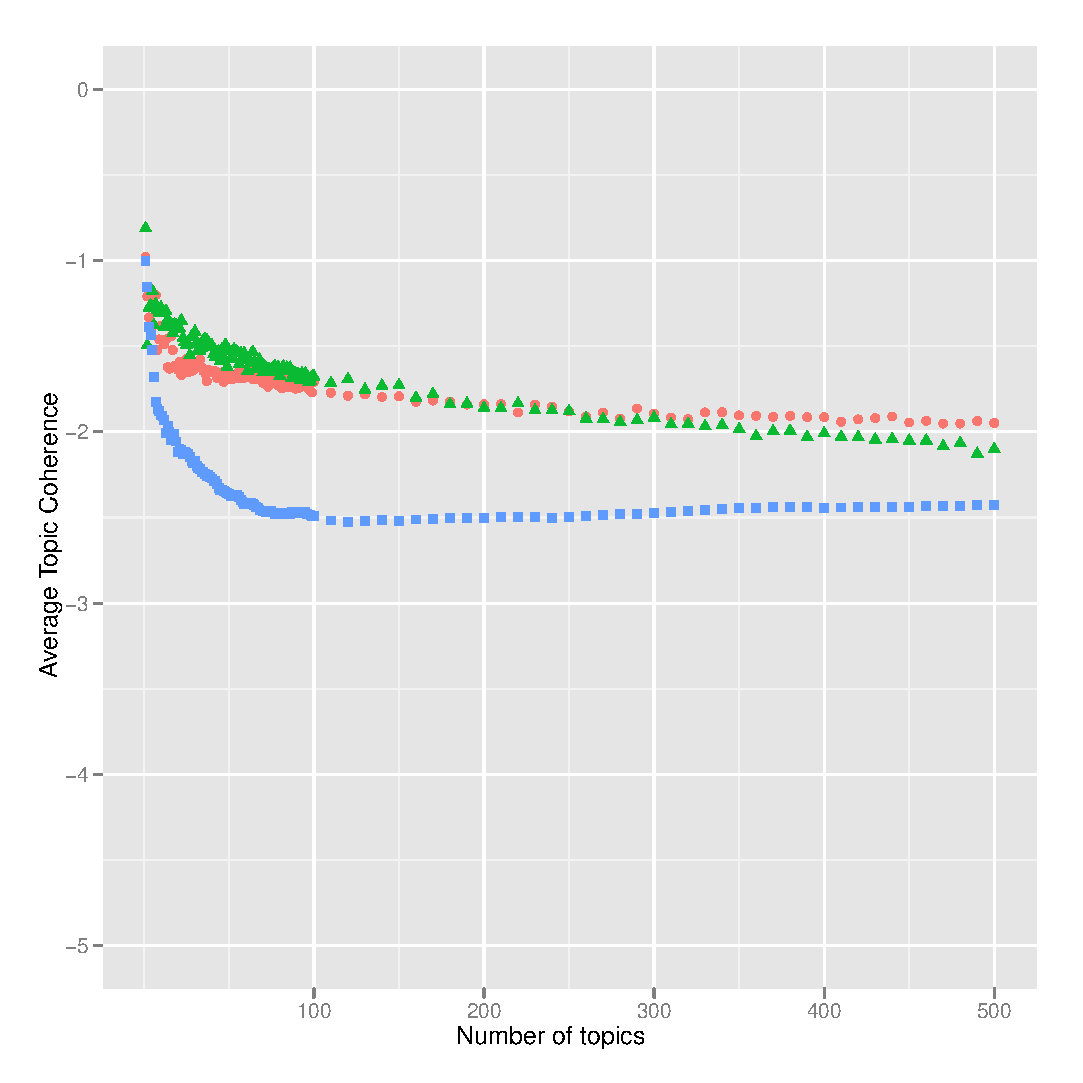
\includegraphics[width=.50\textwidth,height=.35\textwidth]{plots/mean-umass.eps}}
  \subfloat[UCI]{\label{fig:mean-uci}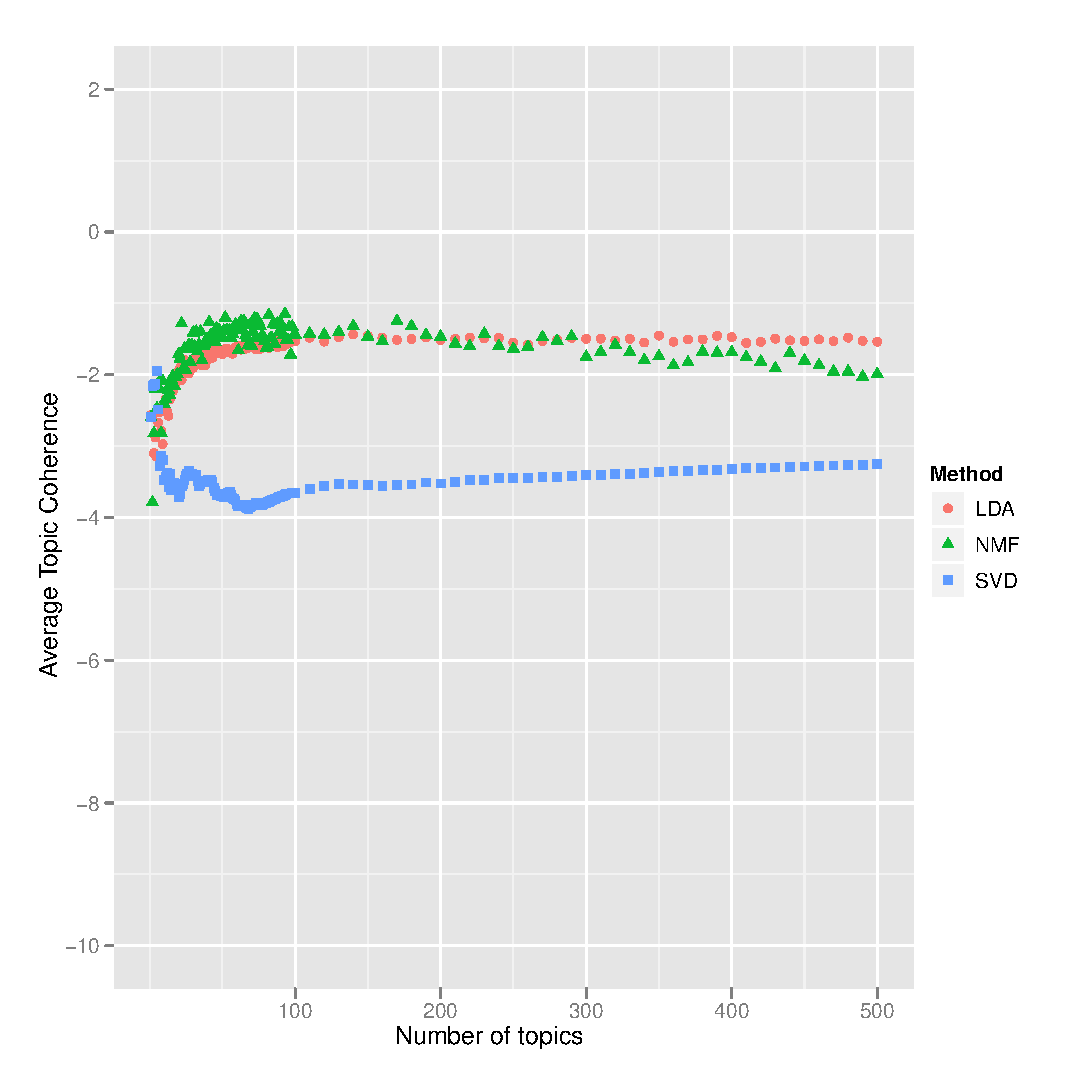
\includegraphics[width=.50\textwidth,height=.35\textwidth]{plots/mean-uci.eps}}
  \caption{Average Topic Coherence for each model}
  \label{fig:mean}
\end{figure*}

\begin{figure*}[h!t!b!]
  \centering
  \subfloat[UMass]{\label{fig:entropy-umass}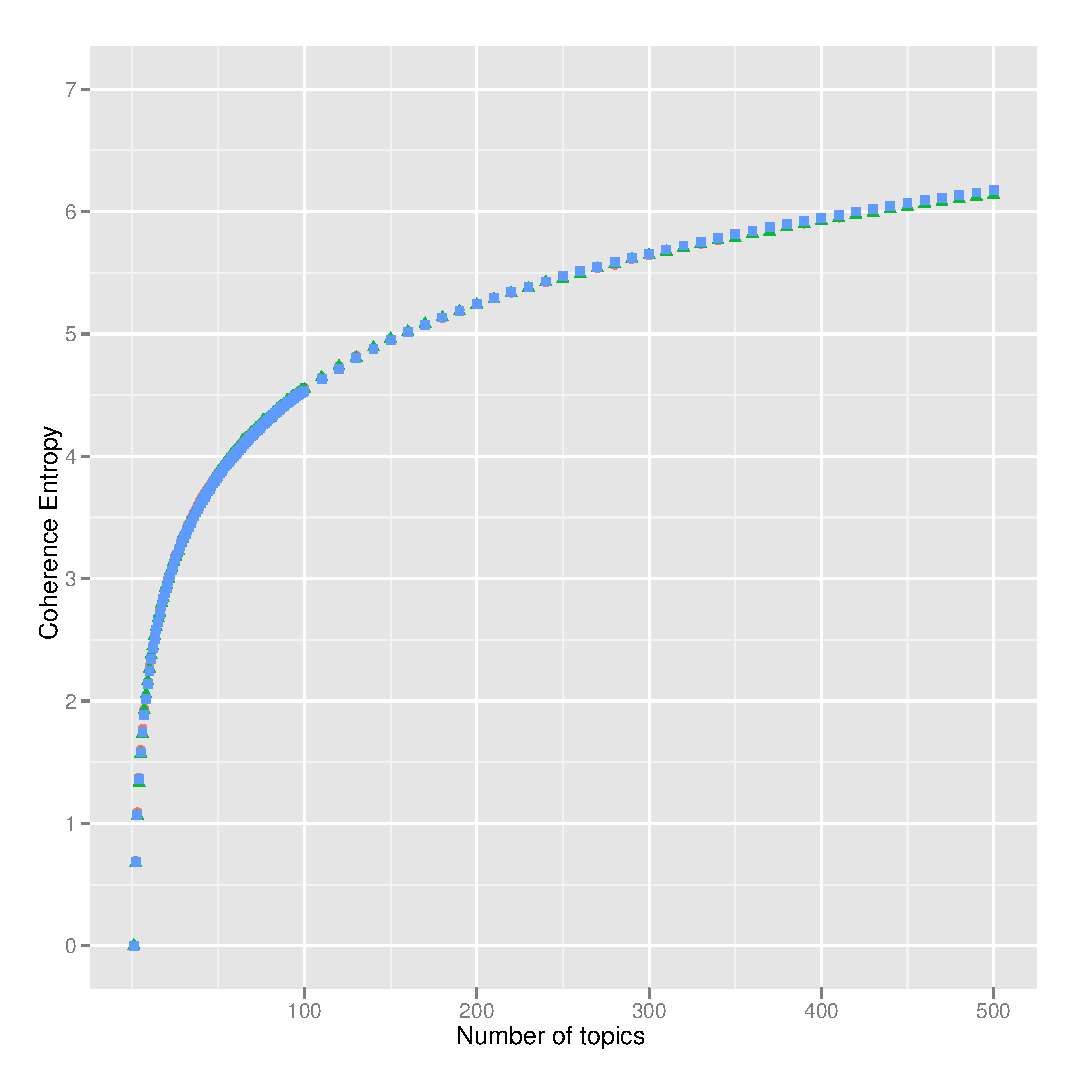
\includegraphics[width=.50\textwidth,height=.35\textwidth]{plots/entropy-umassNoLog.eps}}
  \subfloat[UCI]{\label{fig:entropy-uci}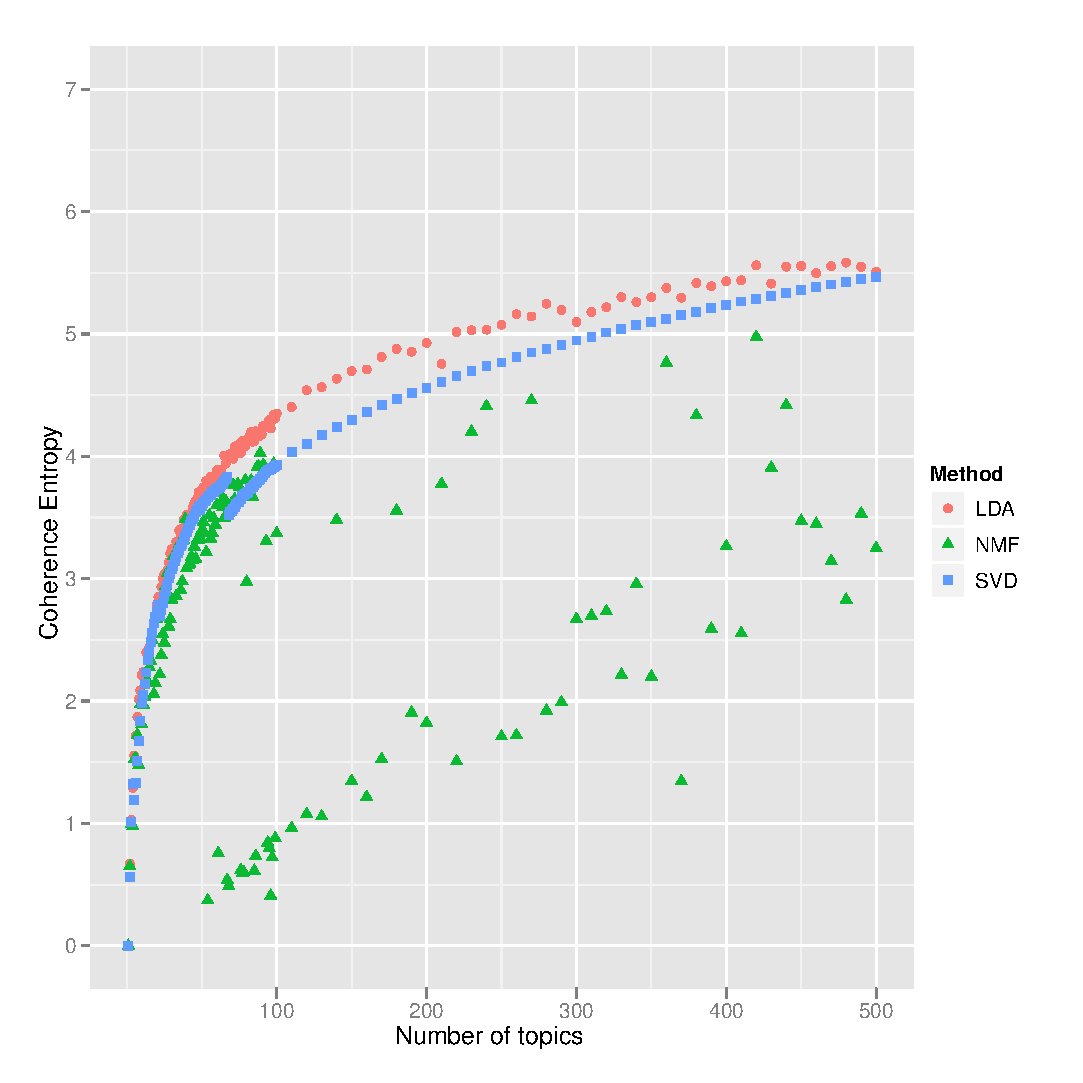
\includegraphics[width=.50\textwidth,height=.35\textwidth]{plots/entropy-uciNoLog.eps}}
  \caption{Entropy of the Topic Coherence for each model}
  \label{fig:entropy}
\end{figure*}

\paragraph{The UMass metric} defines the score to be based on document co-occurrence:

$$score(v_i, v_j,\epsilon) = \log \frac{D(v_i, v_j) + \epsilon}{D(v_j)}$$
\noindent
where $D(x,y)$ counts the number of documents containing words $x$ and $y$ and
$D(x)$ counts the number of documents containing $x$. Significantly, the UMass
metric computes these counts over the \textit{original corpus} used to train the
topic models, rather than an external corpus.  This metric is more intrinsic in
nature.  It attempts to confirm that the models learned data known to be in the
corpus.


\section{Evaluation}
\label{sec:evaluation}
We evaluate the quality of our three topic models (LDA, SVD, and NMF) with three
experiments.  We focus first on evaluating aggregate coherence methods for a complete
topic model and consider the differences between each model as we learn an
increasing number of topics.  Secondly, we compare coherence scores to previous
semantic evaluations.  Lastly, we use the learned topics in a classification
task and evaluate whether or not coherent topics are equally informative when
discriminating between documents.

For all our experiments, we trained our models on 92,600 New York Times articles
from 2003 \cite{nytcorpus}.  For all articles, we removed stop words and any
words occurring less than 200 times in the corpus, which left 35,836 unique
tokens.  All documents were tokenized with OpenNLP's
MaxEnt\footnote{http://incubator.apache.org/opennlp/} tokenizer.  For the UCI
measure, we compute the PMI between words using a 20 word sliding window passed
over the WaCkypedia corpus \cite{baroni09wacky}.  In all experiments, we compute
the coherence with the top 10 words from each topic that had the highest weight,
in terms of LDA and NMF this corresponds with a high probability of the term
describing the topic but for SVD there is no clear semantic interpretation.

\subsection{Aggregate methods for topic coherence}

\begin{figure*}[h!t!b!]
  \centering
  \subfloat[UMass]{\label{fig:mean-umassNoSmooth}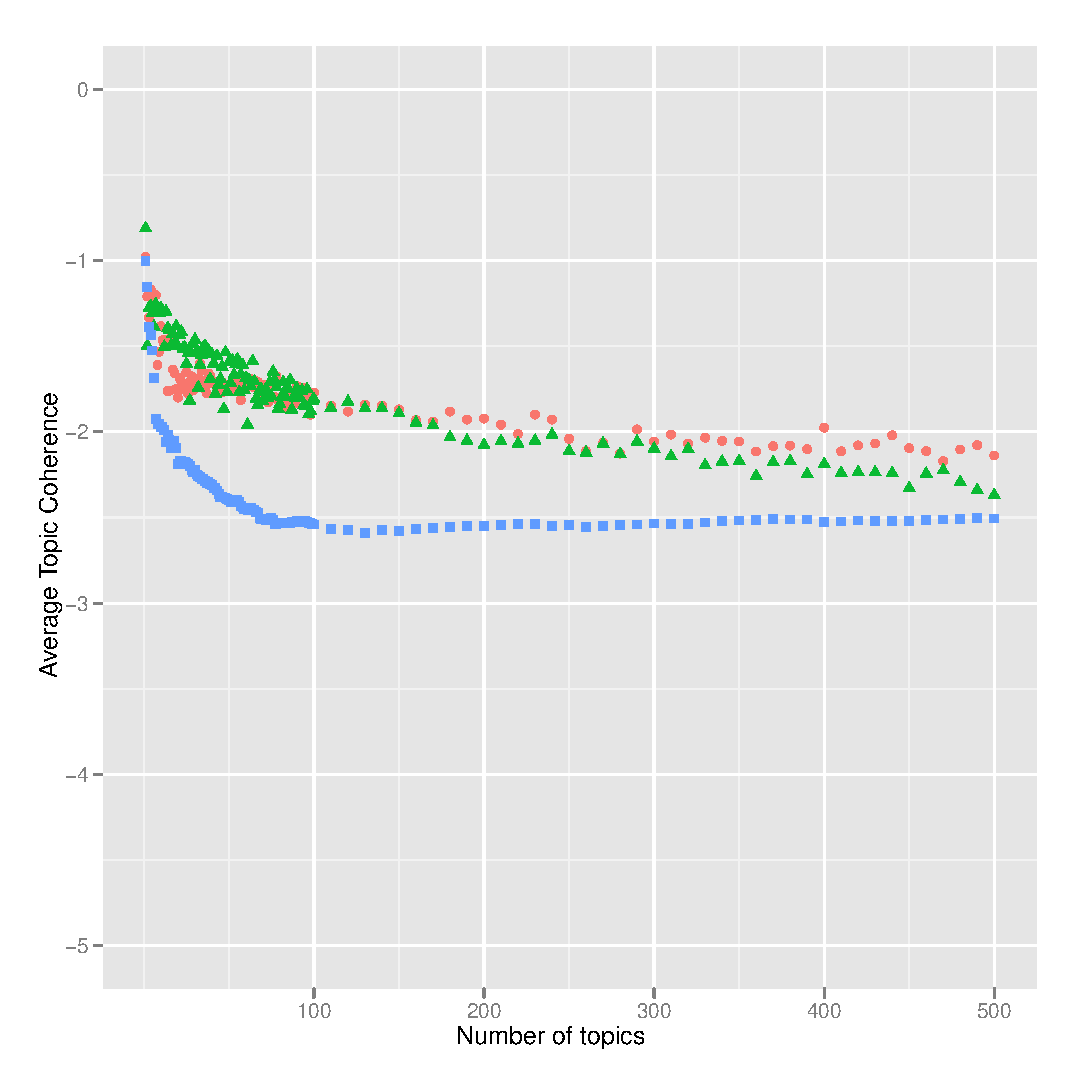
\includegraphics[width=.50\textwidth,height=.35\textwidth]{plots/mean-umassNoSmoothing.eps}}
  \subfloat[UCI]{\label{fig:mean-uciNoSmooth}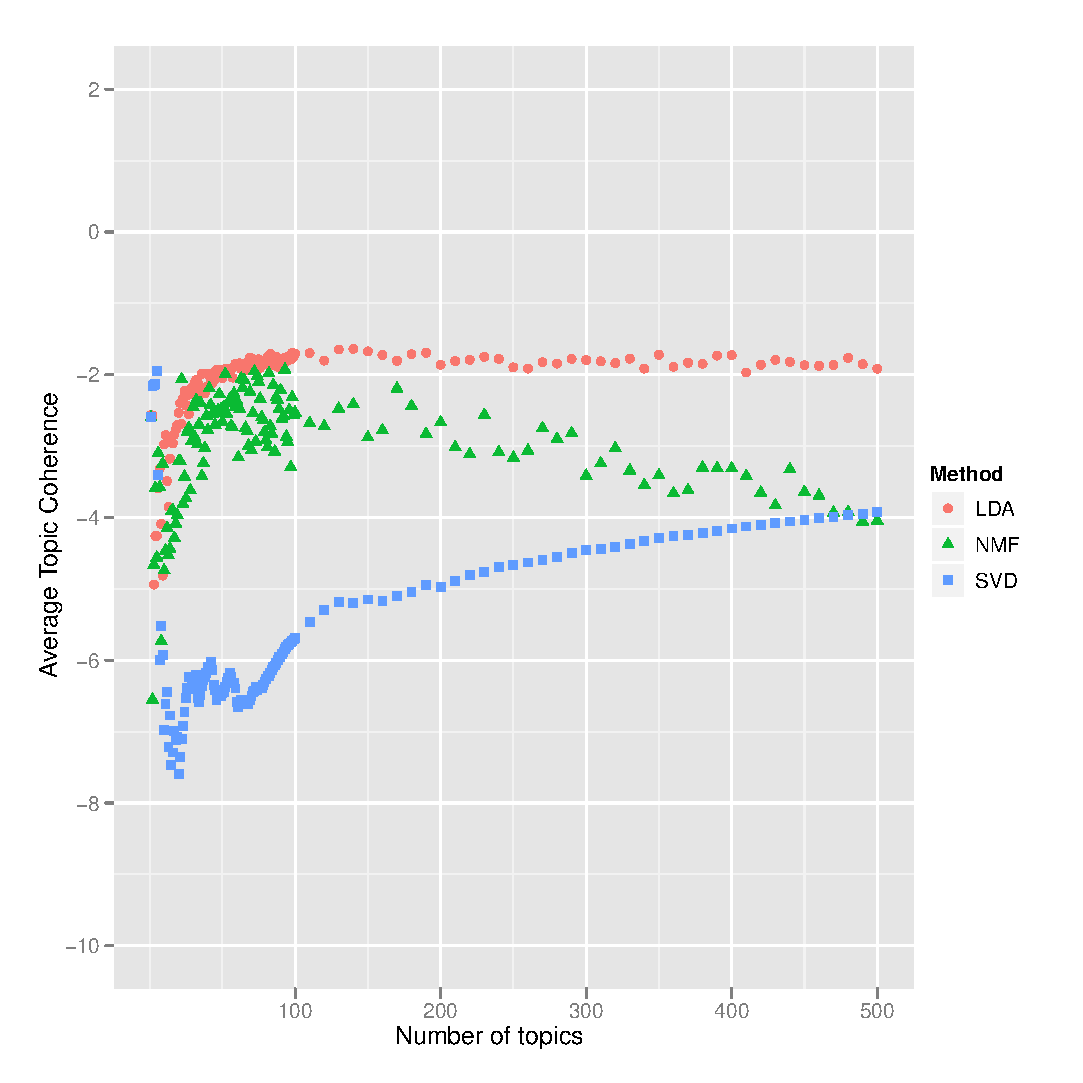
\includegraphics[width=.50\textwidth,height=.35\textwidth]{plots/mean-uciNoSmoothing.eps}}
  \caption{Average Topic Coherence with $\epsilon=10^{-12}$}
  \label{fig:mean-smoothing}
\end{figure*}

\begin{figure*}[h!t!b!]
  \centering
  \subfloat[UMass]{\label{fig:10mean-umassNoSmooth}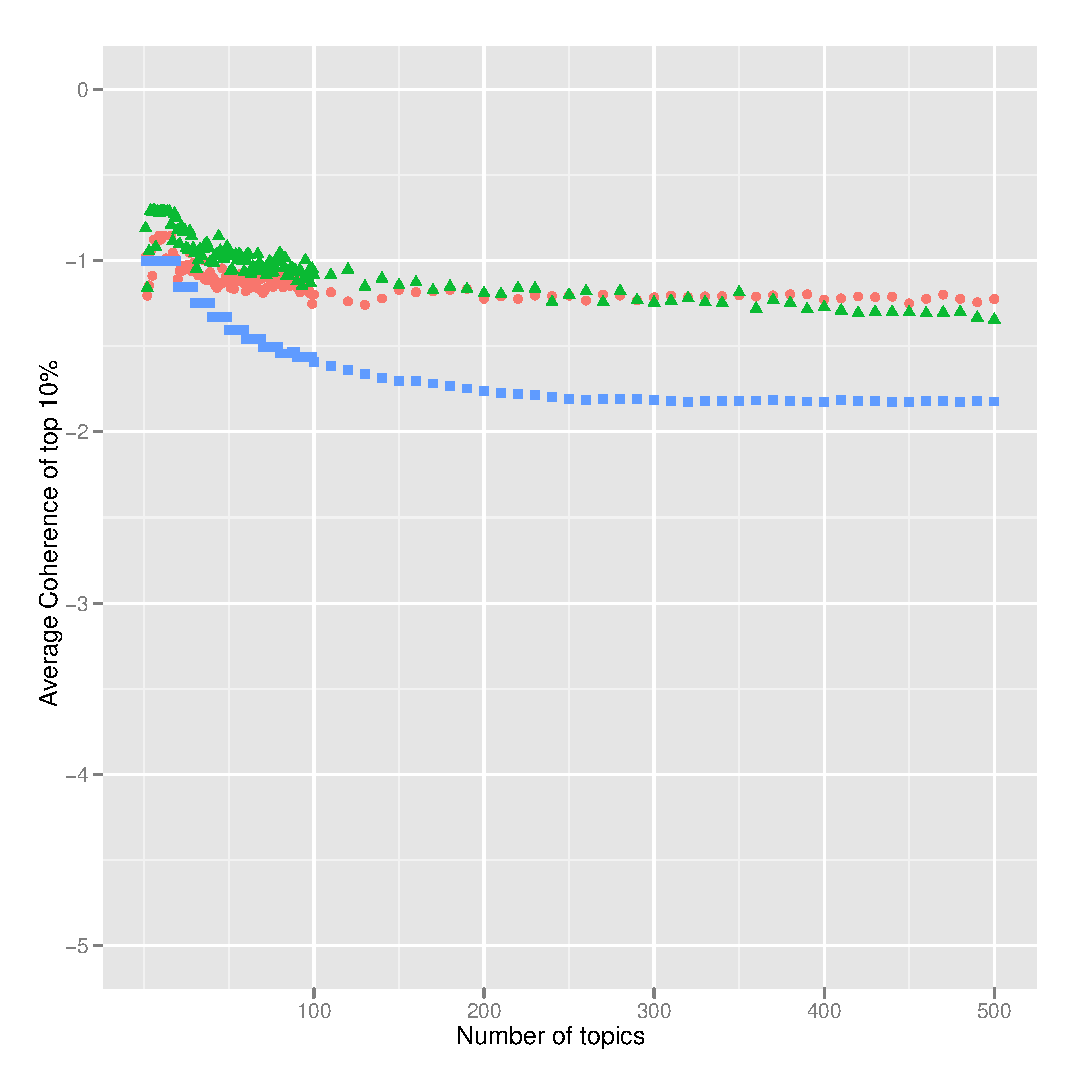
\includegraphics[width=.50\textwidth,height=.35\textwidth]{plots/10mean-umassNoSmoothing.eps}}
  \subfloat[UCI]{\label{fig:10mean-uciNoSmooth}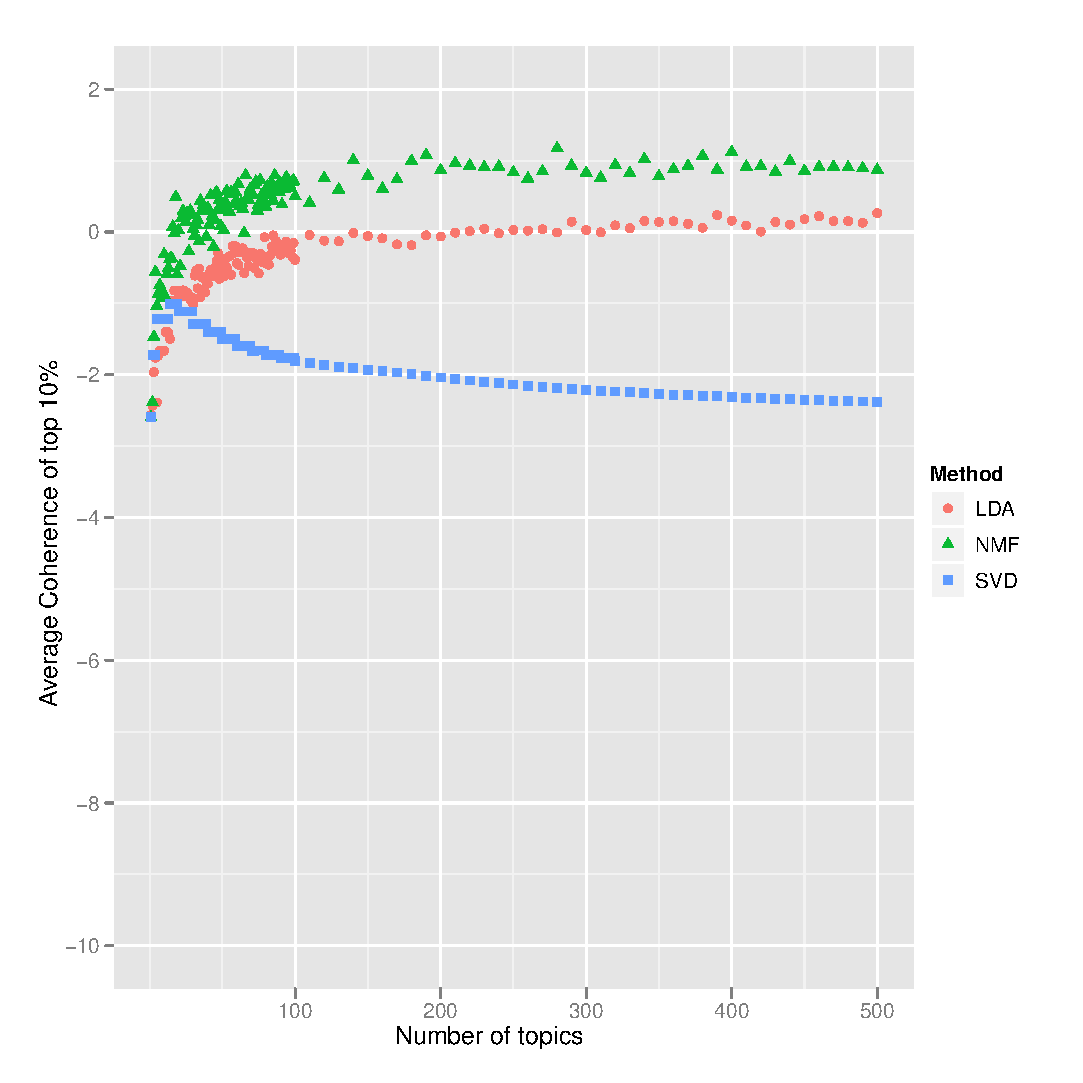
\includegraphics[width=.50\textwidth,height=.35\textwidth]{plots/10mean-uciNoSmoothing.eps}}
  \caption{Average Topic Coherence of the top 10\% topics with $\epsilon=10^{-12}$}
  \label{fig:10mean-smoothing}
\end{figure*}

Before we can compare topic models, we require an aggregate
measure that represents the quality of a complete model, 
rather than individual topics.  We consider two aggregates methods:
(1) the average coherence of all topics and
(2) the entropy of the coherence for all topics.  
The average coherence provides a quick summarization of a model's quality
whereas the entropy provides an alternate summarization that differentiates
between two interesting situations.  Since entropy measures the complexity of a
probability distribution, it can easily differentiate between uniform
distributions and multimodal, distributions.  This distinction is relevant when
users prefer to have roughly uniform topic quality instead of a wide gap between
high- and low-quality topics, or vice versa.  We compute the entropy by dropping
the $log$  and $\epsilon$ factor from each scoring function.

Figure \ref{fig:mean} shows the average coherence scores for each model as we
vary the number of topics.  These average scores indicate some simple
relationships between the models: LDA and NMF have approximately the same
performance and both models are consistently better than SVD.  All of the models
quickly reach a stable average score at around 100 topics.  This initially
suggests that learning more topics neither increases or decreases the quality of
the model, but Figure \ref{fig:entropy} indicates otherwise.  While the entropy
for the UMass score stays stable for all models, NMF produces erratic entropy
results under the UCI score as we learn more topics.  As entropy is higher for
even distributions and lower for all other distributions, these results suggest
that the NMF is learning topics with drastically different levels of quality,
i.e. some with high quality and some with very low quality, but the average
coherence over all topics do not account for this.

\begin{comment}
\begin{figure*}[h!t!b!]
  \centering
  \subfloat[UMass]{\label{fig:ordered-umassNoSmooth}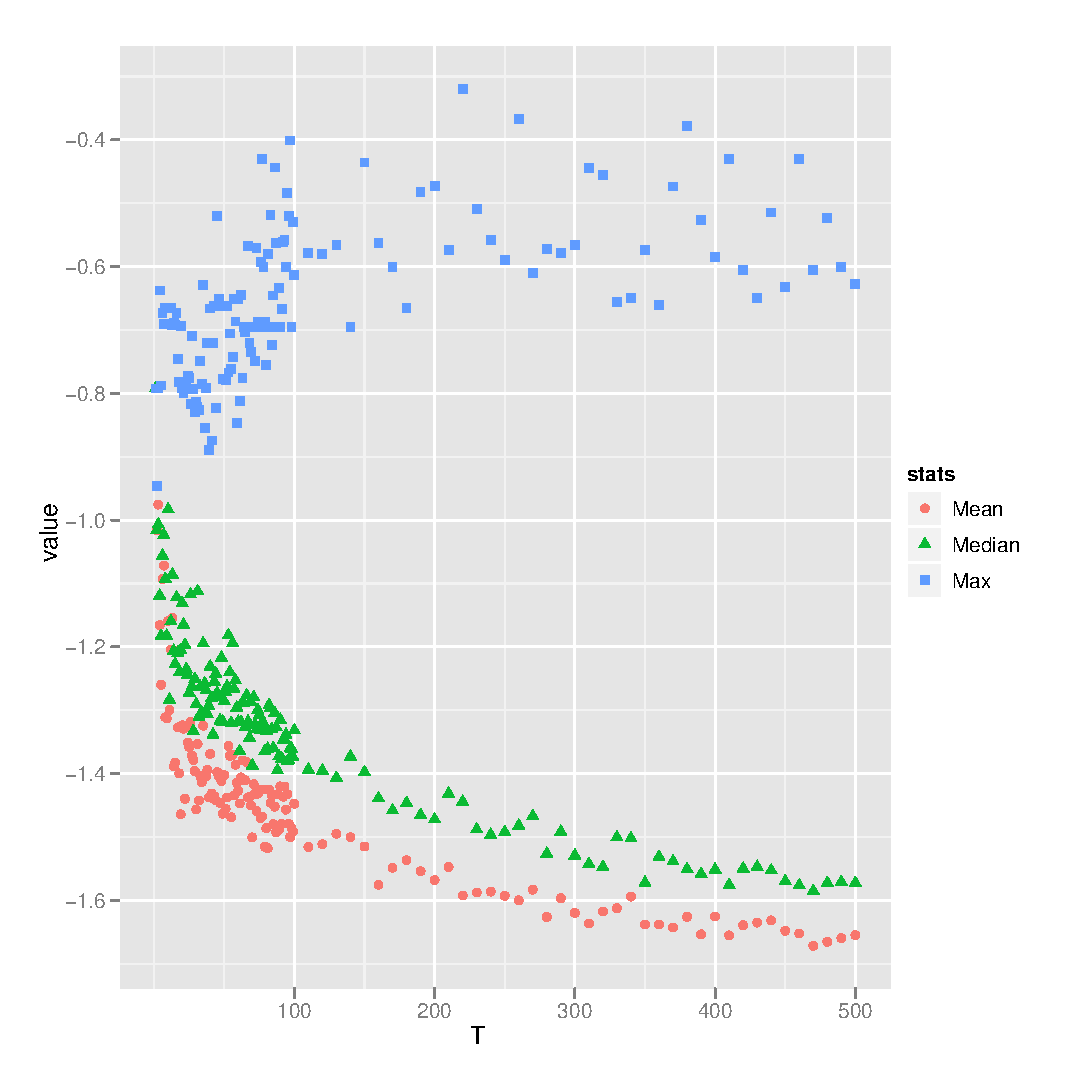
\includegraphics[width=.50\textwidth,height=.35\textwidth]{plots/lda-nmf-umass.eps}}
  \subfloat[UCI]{\label{fig:ordered-uciNoSmooth}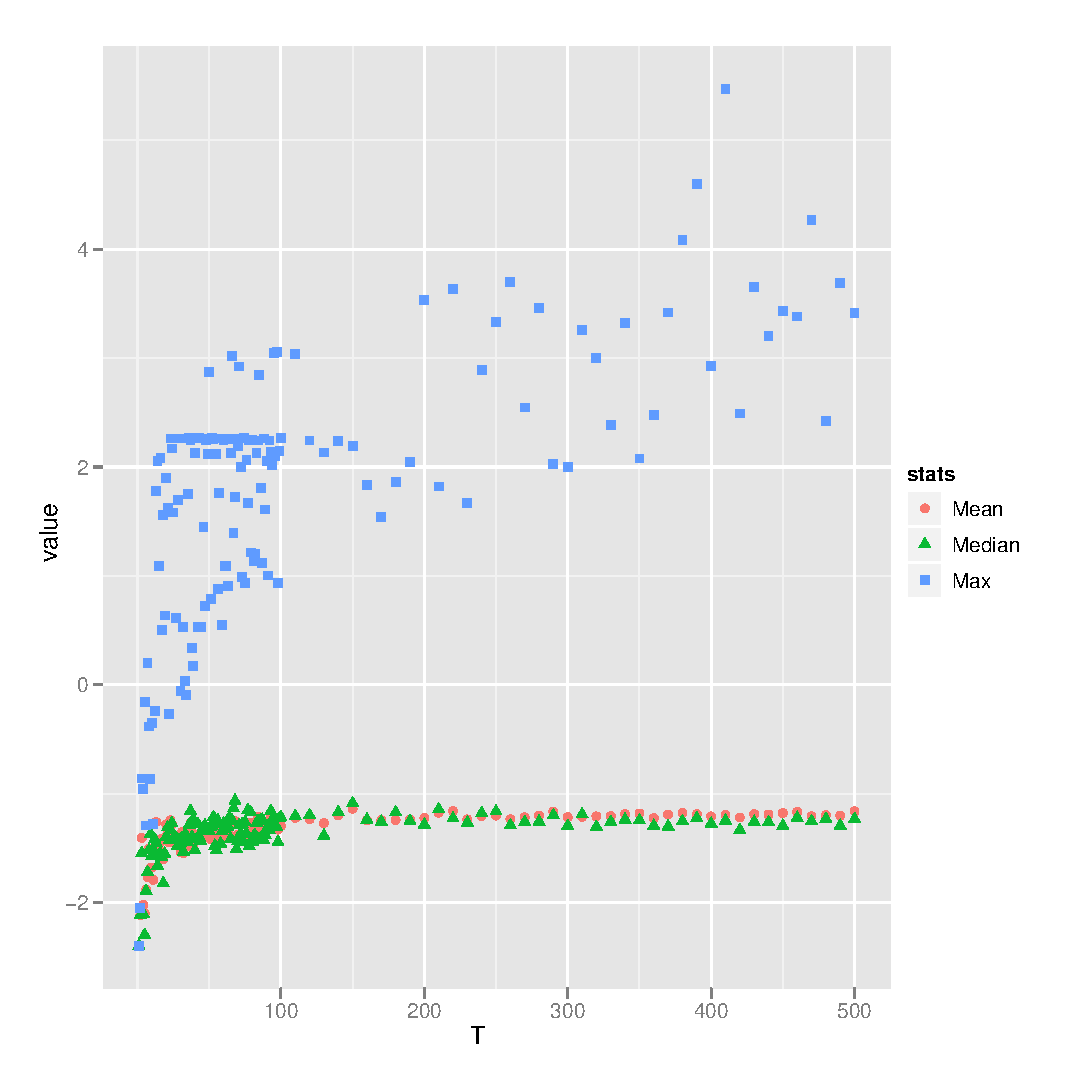
\includegraphics[width=.50\textwidth,height=.35\textwidth]{plots/lda-nmf-uci.eps}}
  \caption{Bipartite weights between LDA and NMF models using the Hungarian Algorithm}
  \label{fig:paired-weights}
\end{figure*}

\begin{figure*}[h!t!b!]
  \centering
  \subfloat[UMass]{\label{fig:ordered-umassNoSmooth}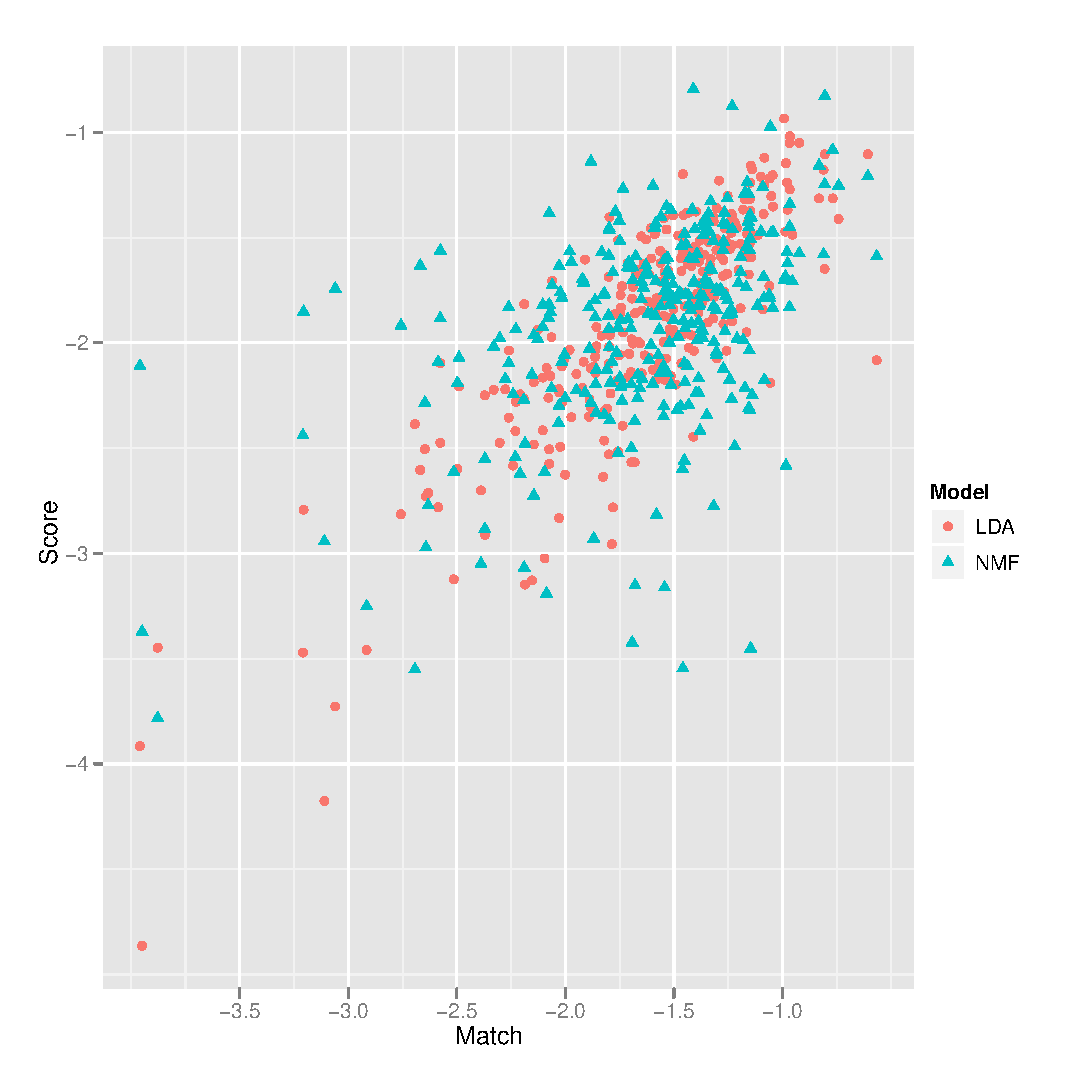
\includegraphics[width=.50\textwidth,height=.35\textwidth]{plots/lda-nmf-umass-300.eps}}
  \subfloat[UCI]{\label{fig:ordered-uciNoSmooth}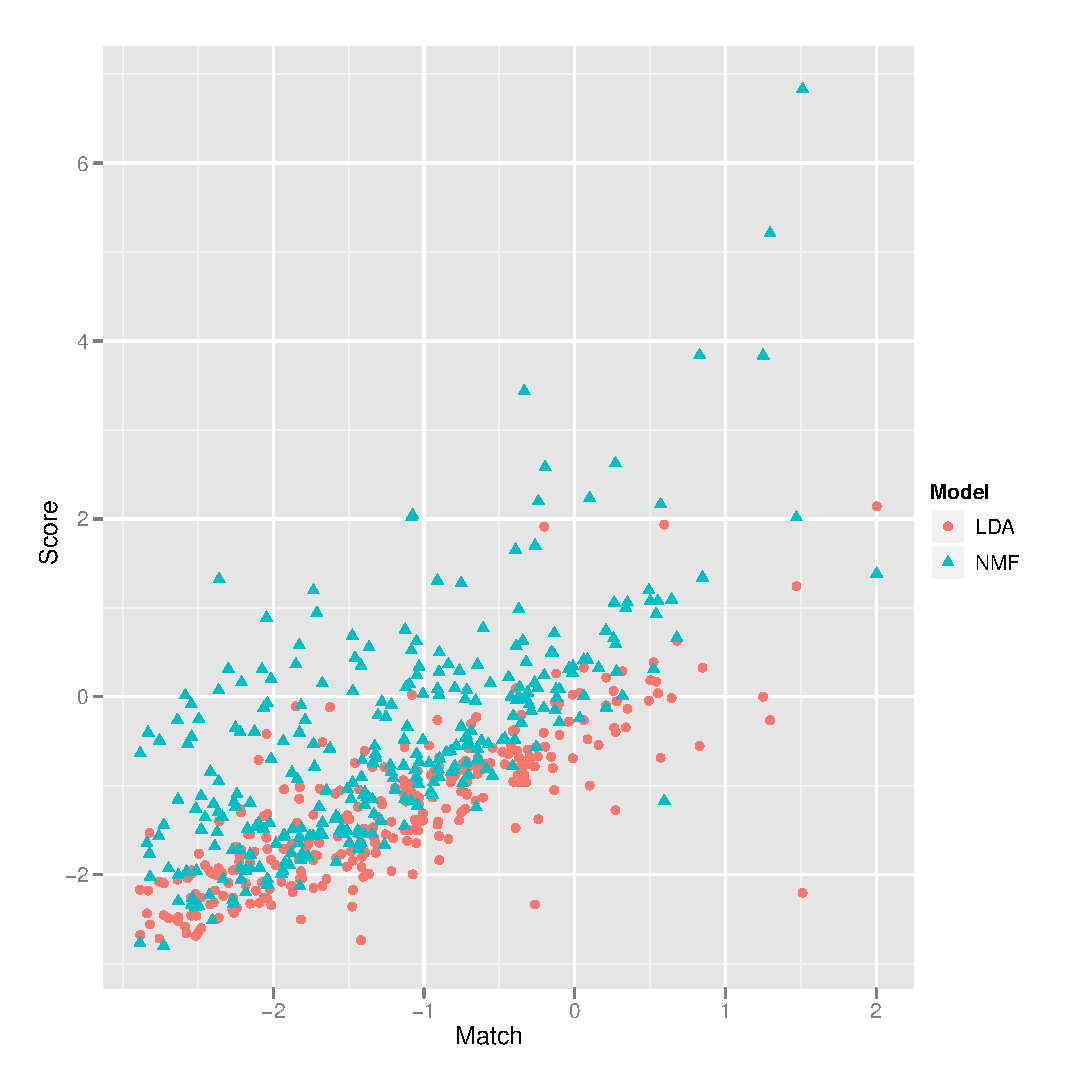
\includegraphics[width=.50\textwidth,height=.35\textwidth]{plots/lda-nmf-uci-300.eps}}
  \caption{Relation between bipartite weights and topic coherence scores for 300 topics}
  \label{fig:score-weight-300}
\end{figure*}
\end{comment}

\begin{figure*}[h!t!b!]
  \centering
  \subfloat[Rubenstein \&
  Goodenough]{\label{fig:rng-wordsim}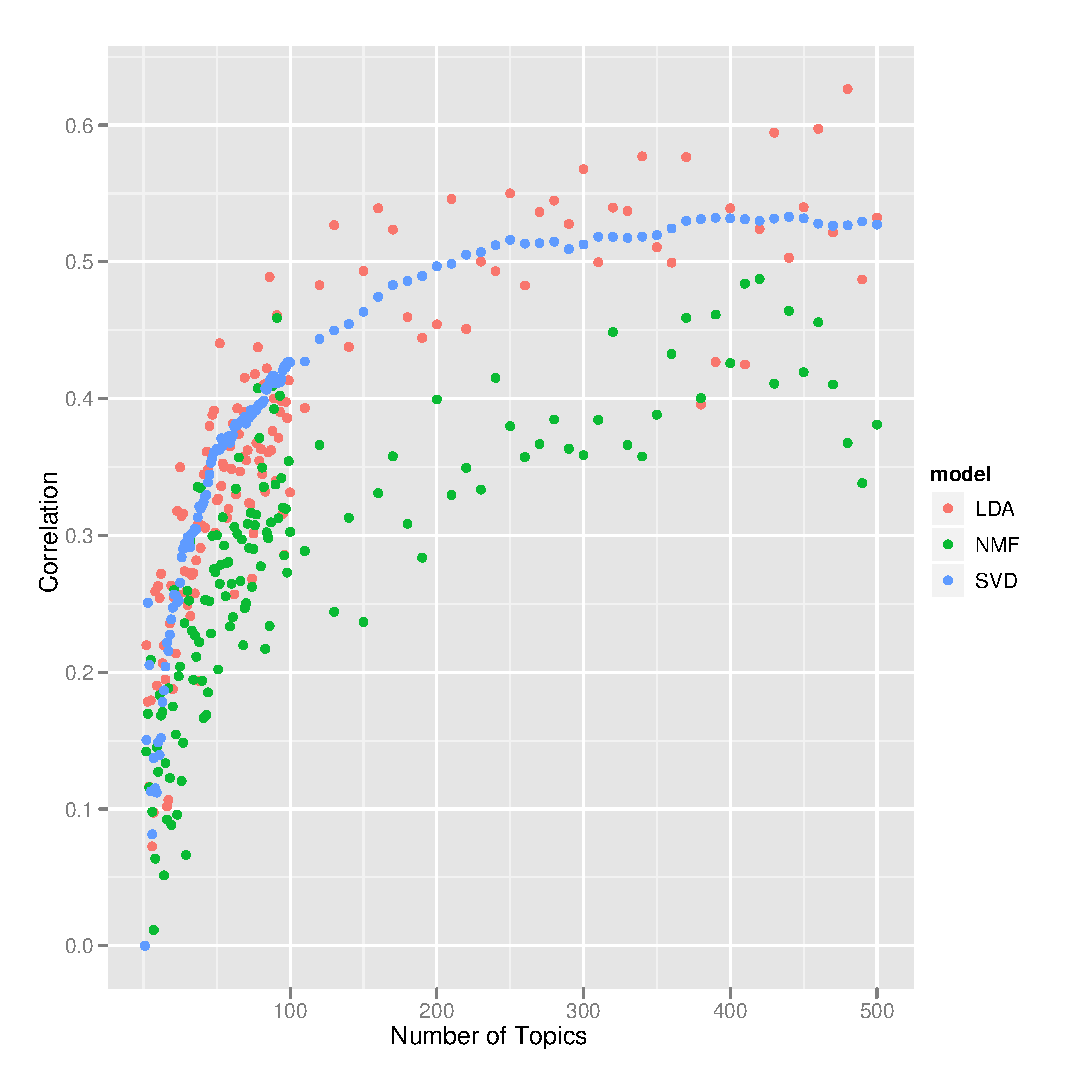
\includegraphics[width=.50\textwidth,height=.35\textwidth]{plots/rng_wordsim.eps}}
  \subfloat[Wordsim
  353/Finklestein~et.~al.]{\label{fig:353-wordsim}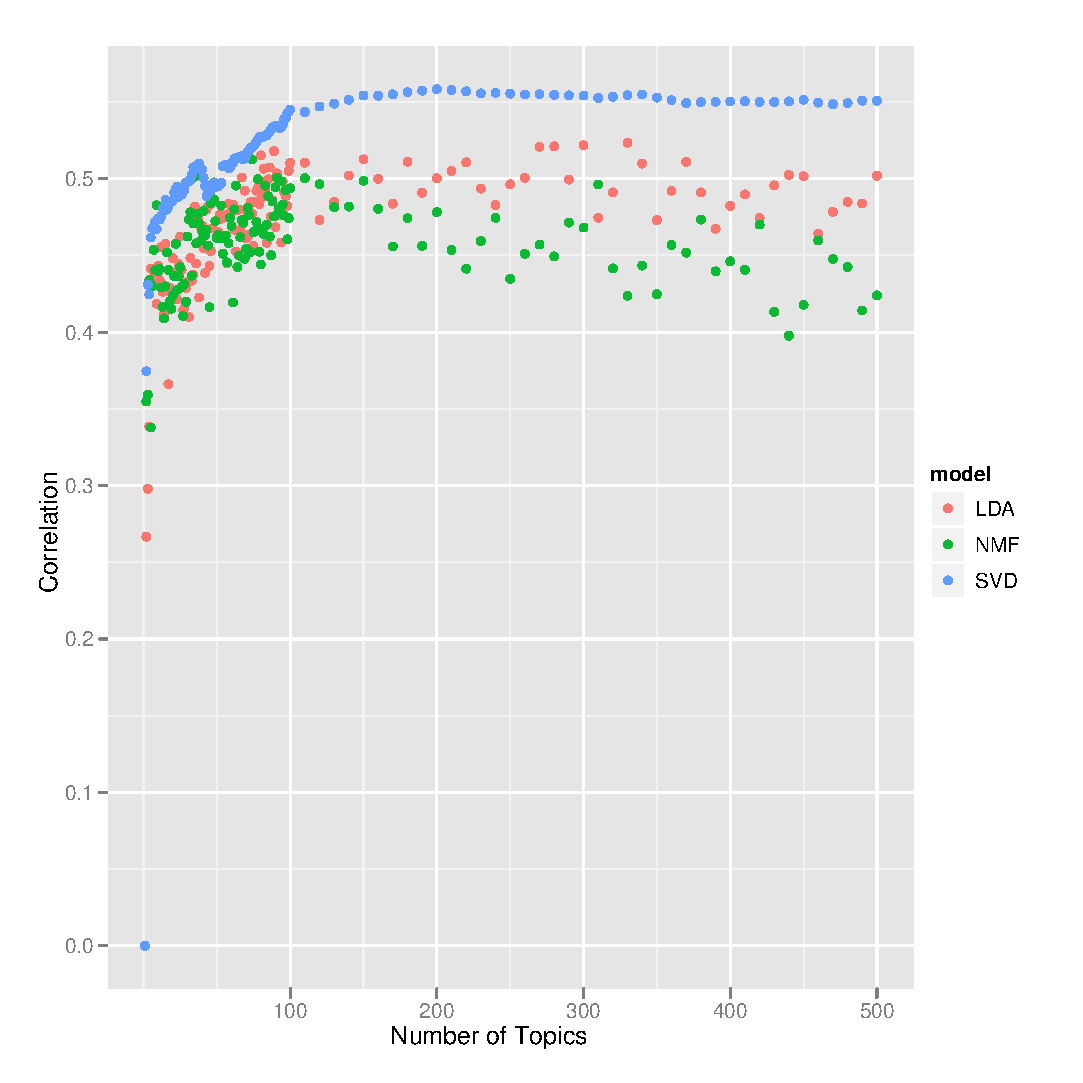
\includegraphics[width=.50\textwidth,height=.35\textwidth]{plots/353_wordsim.eps}}
  \caption{Word Similarity Evaluations for each model}
  \label{fig:wordsim}
\end{figure*}

\begin{figure}[h!t!b!]
  \centering
  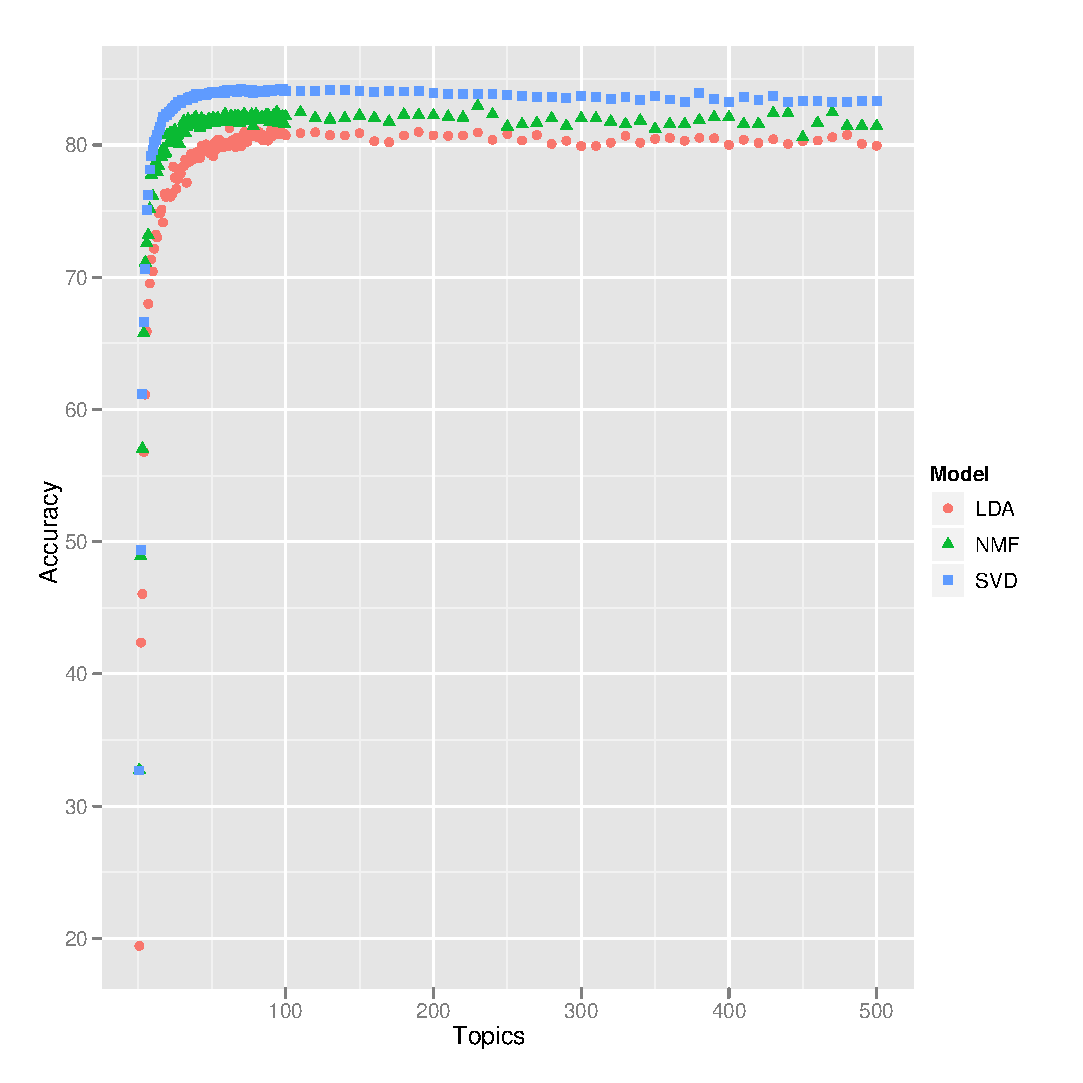
\includegraphics[width=.50\textwidth,height=.35\textwidth]{plots/avatar_classifier.eps}
  \caption{Classification accuracy for each model}
  \label{fig:predict}
\end{figure}

Low quality topics may be composed of highly unrelated words that
can't be fit into another topic, and in this case, our smoothing
factor, $\epsilon$, may be artificially increasing the score for
unrelated words. Following the practice of the original use of these
metrics, in Figures~\ref{fig:mean} and \ref{fig:entropy} we set
$\epsilon = 1$. In Figure~\ref{fig:mean-smoothing}, we consider
$\epsilon = 10^{-12}$, which should significantly reduce the score for
completely unrelated words. Here, we see a significant change in the
performance of NMF, the average coherence decreases dramatically as we
learn more topics. Similarly, performance of SVD drops dramatically
and well below the other models. In figure \ref{fig:10mean-smoothing}
we lastly compute the average coherence using only the top 10\% most
coherence topics with $\epsilon = 10^{-12}$. Here, NMF again performs
on par with LDA. With the top 10\% topics still having a high average
coherence but the full set of topics having a low coherence, NMF
appears to be learning more low quality topics once it's learned the
first 100 topics, whereas LDA learns fewer low quality topics in
general.

\begin{comment}
\begin{figure*}
  \centering
  \subfloat[UMass]{\label{fig:ordered-umass}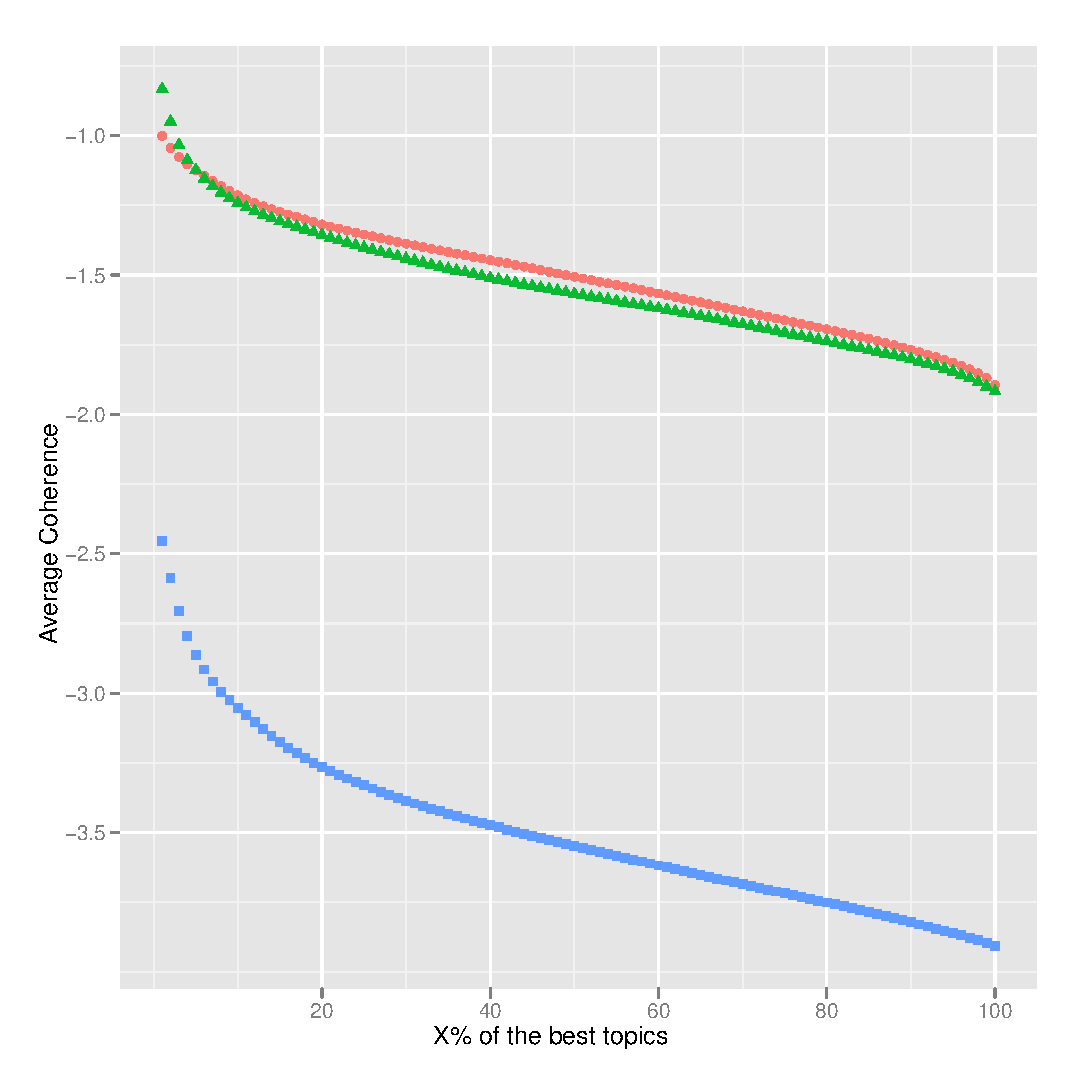
\includegraphics[width=.50\textwidth,height=.35\textwidth]{plots/ordered_300_umass.eps}}
  \subfloat[UCI]{\label{fig:ordered-uci}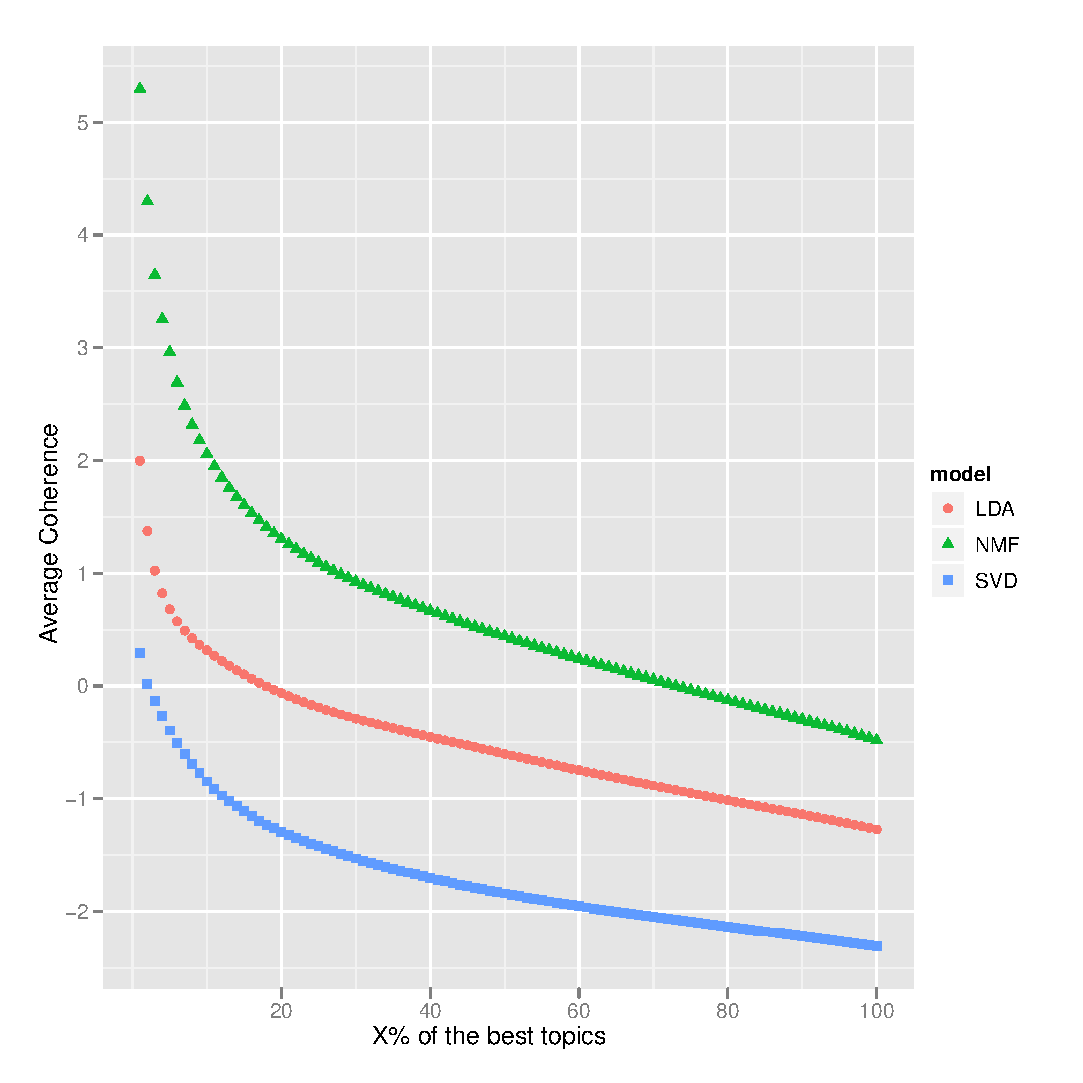
\includegraphics[width=.50\textwidth,height=.35\textwidth]{plots/ordered_300_uci.eps}}
  \caption{Topic Coherence for the top X\% topics out of 300 topics}
  \label{fig:top10avg}
\end{figure*}

\begin{figure*}
  \centering
  \subfloat[UMass]{\label{fig:ordered-umassNoSmooth}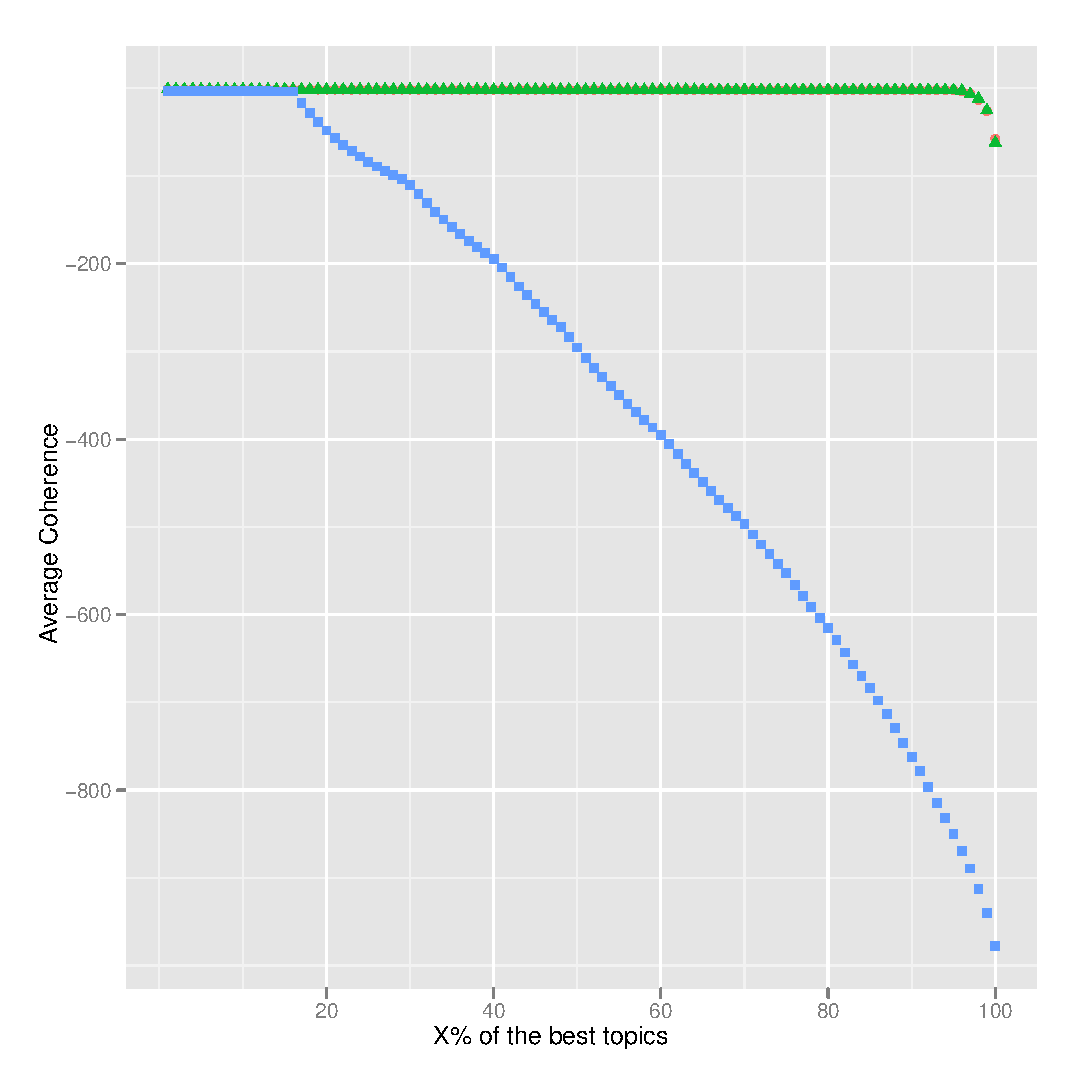
\includegraphics[width=.50\textwidth,height=.35\textwidth]{plots/ordered_300_umassNoSmoothing.eps}}
  \subfloat[UCI]{\label{fig:ordered-uciNoSmooth}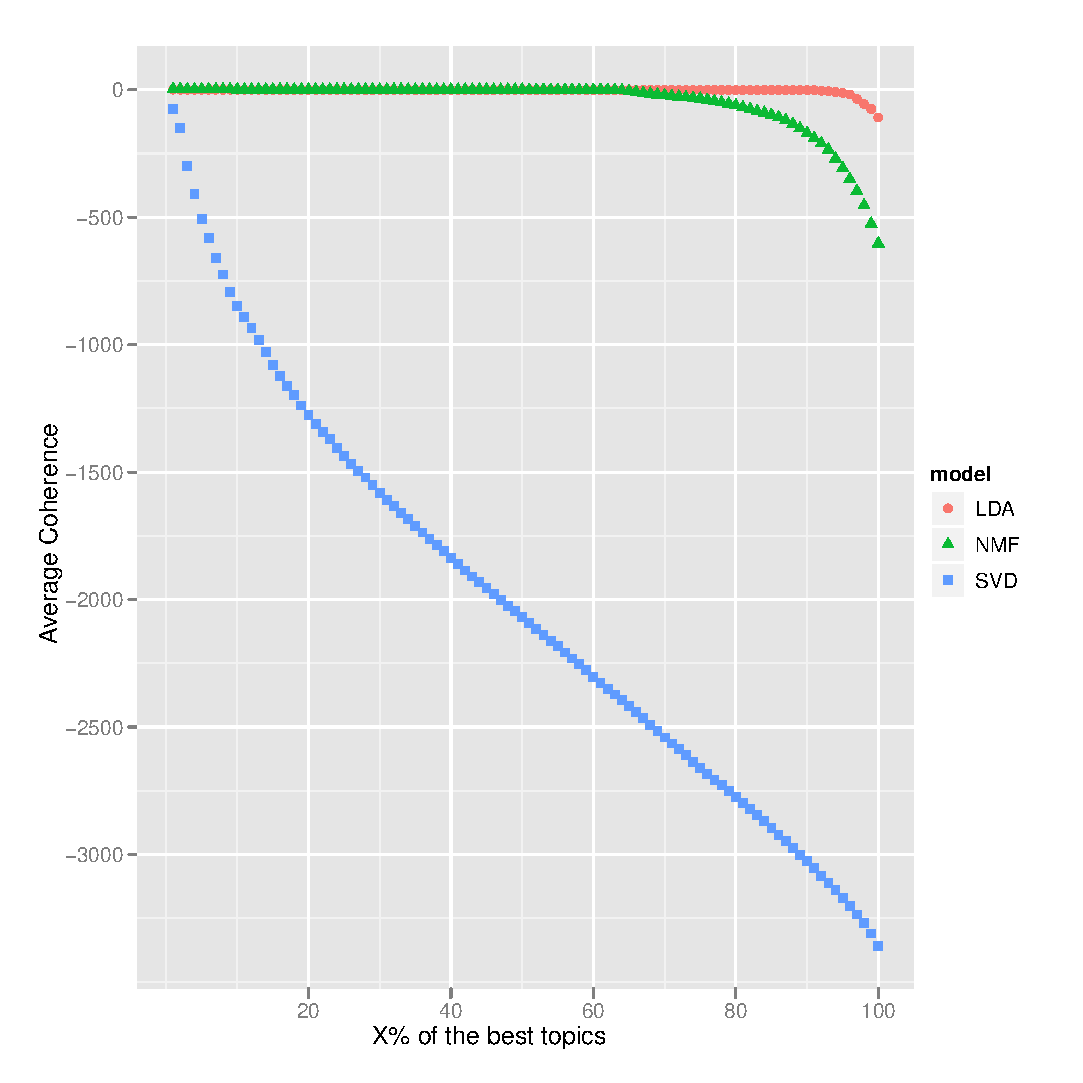
\includegraphics[width=.50\textwidth,height=.35\textwidth]{plots/ordered_300_uciNoSmoothing.eps}}
  \caption{Topic Coherence for the top X\% topics out of 300 topics with $\epsilon=10^{-12}$}
  \label{fig:top10avg}
\end{figure*}

\begin{figure}
  \centering
  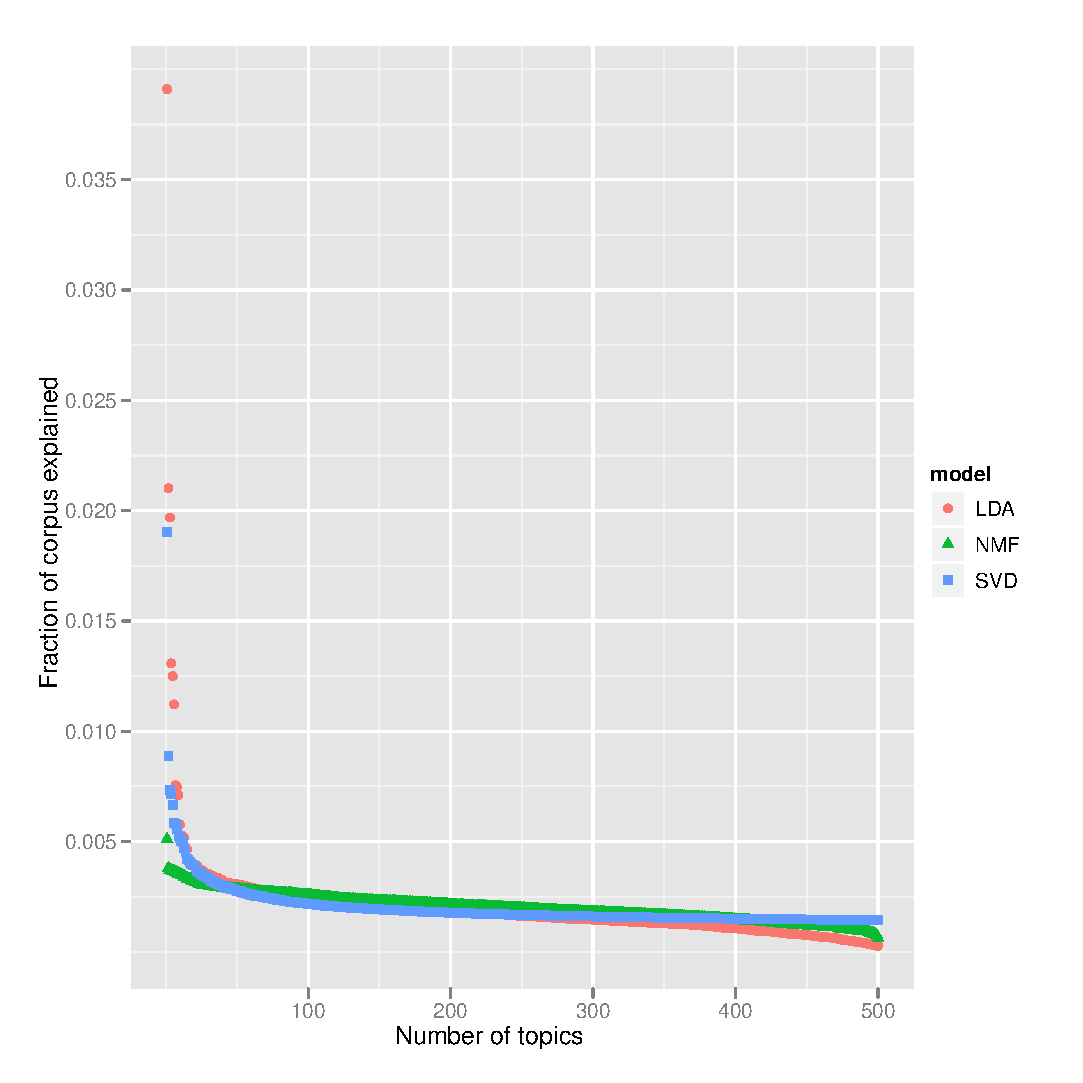
\includegraphics[width=.50\textwidth,height=.35\textwidth]{plots/model_topic_probs.eps}
  \caption{The inherent strength of each topic in descending order}
  \label{fig:topicProbs}
\end{figure}
\end{comment}

\begin{comment}
\subsection{Matching Topics}

In the previous experiment, LDA and NMF regularly produced the most coherent
topics, thus.  With such similar scores, we wish to know whether or not the two
models are learning similar topics.  For example, are the best 10 topics from
LDA equivalent to the best 10 topics from NMF?  To address this possibility, we
find the coherence between a pair of topics, $V$ and $Z$ with the following
measure:

$$pairCoherence(V, Z) = \sum_{v_i \in V, z_j \in Z} score(v_i, z_i)$$

Now, we can compare the coherence, or relatedness, between topics
between two models by first comparing the $pairCoherence$ between all topic
combinations between two models and then finding the best matching topics with
the Hungarian Algorithm, which finds an optimal bipartite matching.  If two
models are learning the same topics, we would expect the best matching to be
high, otherwise we can be confidence that the two models are learning unique
sets of topics, and thus users could potentially use both models.

\begin{table}[h]
\footnotesize
\center
\begin{tabular}{|c|c|p{1.75in}|}
\hline
Quality & Model & Topic Terms \\
\hline
\multirow{2}{*}{Best}
& LDA & wine wines bottle grapes made winery cabernet grape pinot red \\
& NMF & tannins chardonnay sauvignon wine 2000 vintages tasting merlot cabernet wines \\
\hline
\multirow{2}{*}{Worst}
& LDA & page front paper article news writer 24 16 28 read \\
& NMF & lists designations 3 7 serials boy 2 witchcraft 8 paperbacks \\
\hline
\end{tabular}
\label{tab:match-words}
\caption{The top 10 words from the best and worst matching topics from LDA and
NMF}
\end{table}

We show the $pairCoherence$ scores first in Figure
\ref{fig:paired-weights} using both coherence scoring methods.  This plots the
best, the average, and the median matching scores between LDA and NMF as we
learn a variable number of topics.  The maximum scores show that both LDA and
NMF are learning at least one highly similar topic.  Consider the best paired
topics from LDA and NMF when using the UCI measure in table
\ref{tab:match-words}.  Here, both models clearly learned a topic about wines
and wine making.  Also as expected, the two least connected topics have no
noticeable connection.  Furthermore, the medians and averages indicate that the
rest of the topics are also mutually coherent.  

We last consider the relation between $pairCoherence$ and the topic coherence
for the topics from each model.  Figure \ref{fig:score-weight-300} makes this
comparison directly for each model.  Under both measures the $pairCoherence$ and
topic coherence show a clear but somewhat weak correlation, as the
$pairCoherence$ increases, so does the topic coherence, especially for the best
matched topics.  

\end{comment}
\subsection{Word Similarity Tasks}

\begin{figure*}[h!t!b!]
  \centering
  \subfloat[UMass]{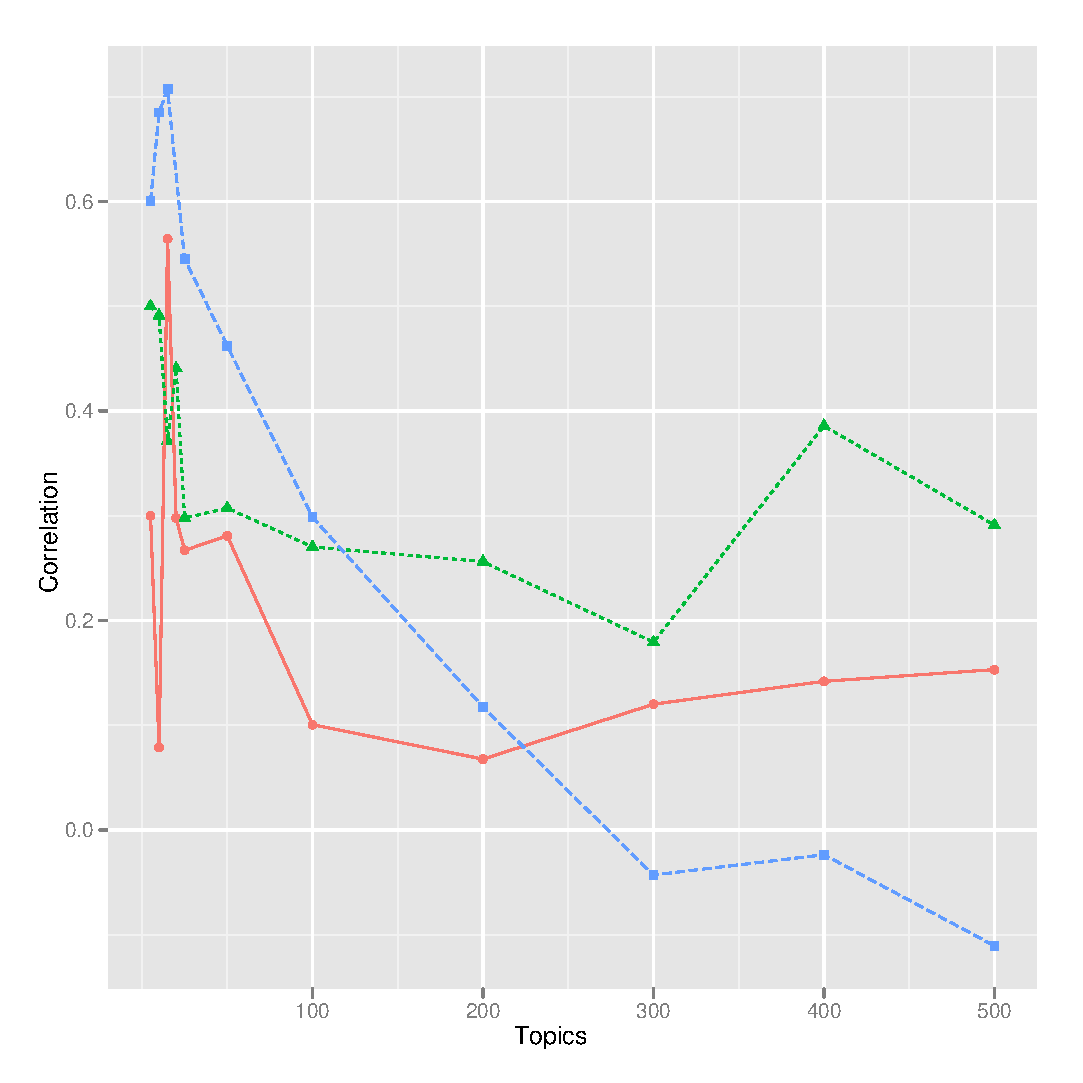
\includegraphics[width=.50\textwidth,height=.35\textwidth]{plots/umassNoSmoothing-ranks.eps}}
  \subfloat[UCI]{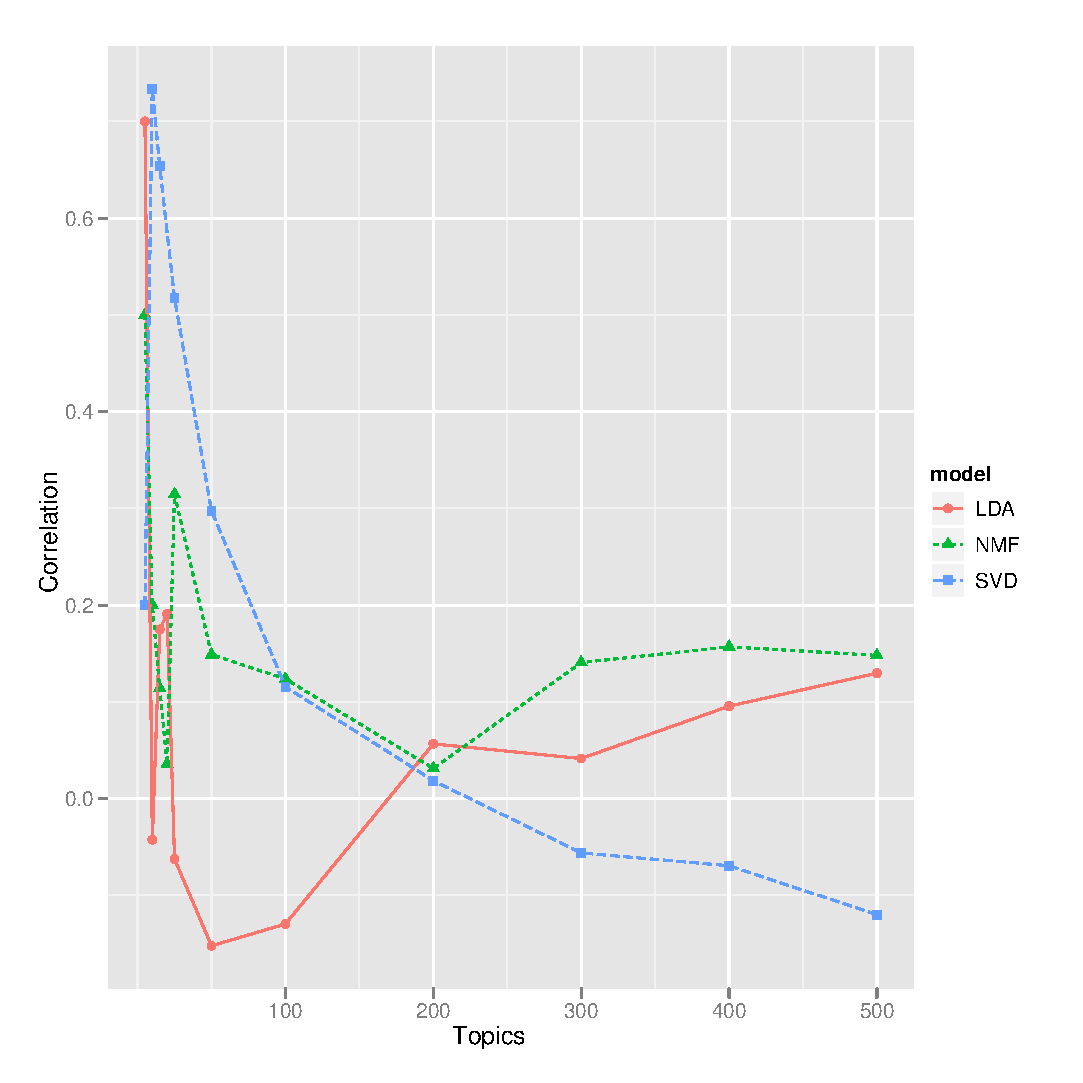
\includegraphics[width=.50\textwidth,height=.35\textwidth]{plots/uciNoSmoothing-ranks.eps}}
  \caption{Correlation between topic coherence and topic ranking in
  classification}
  \label{fig:topic-ranks}
\end{figure*}

\begin{figure*}[h!t!b!]
  \centering
  \subfloat[UMass]{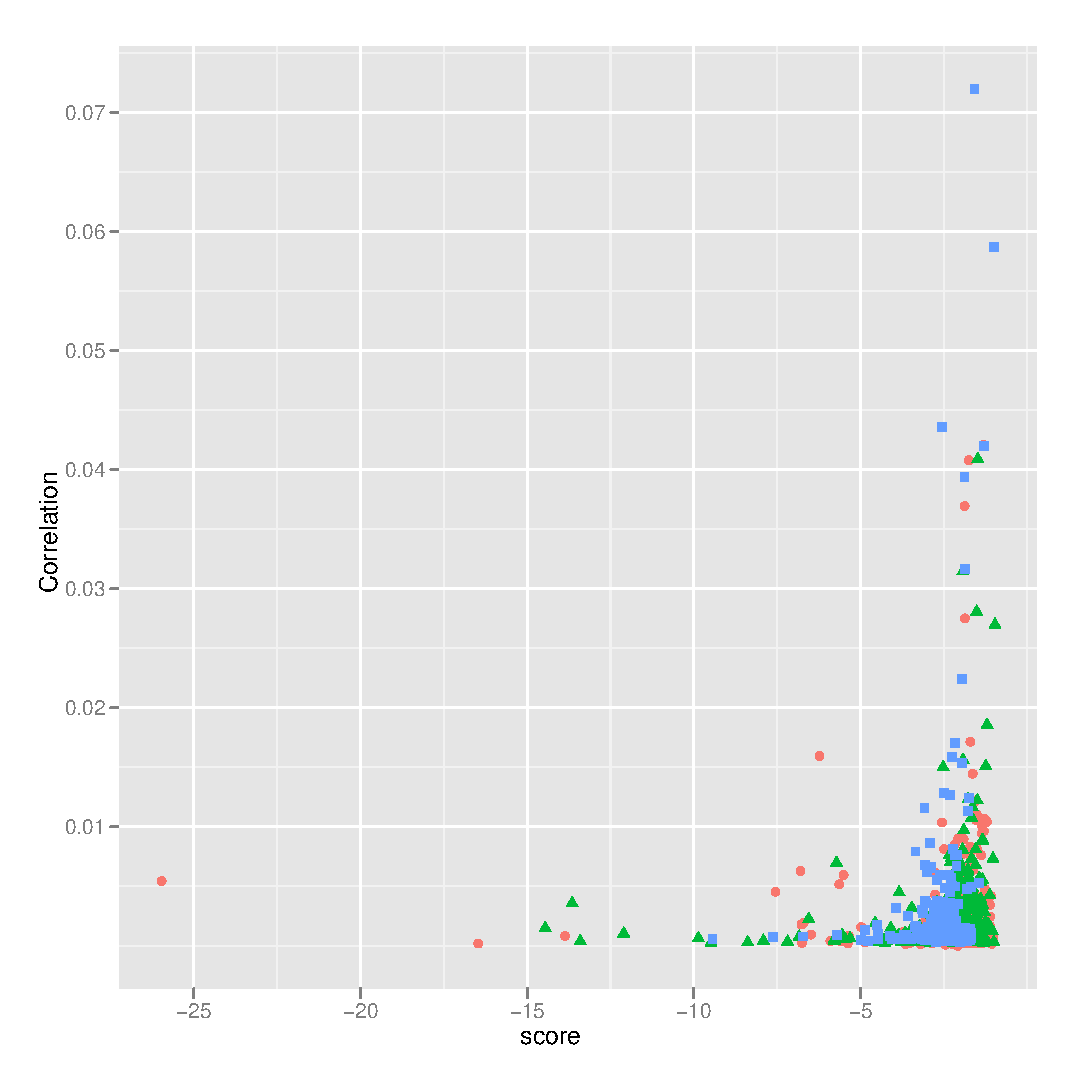
\includegraphics[width=.50\textwidth,height=.35\textwidth]{plots/umassNoSmoothing-rank-500.eps}}
  \subfloat[UCI]{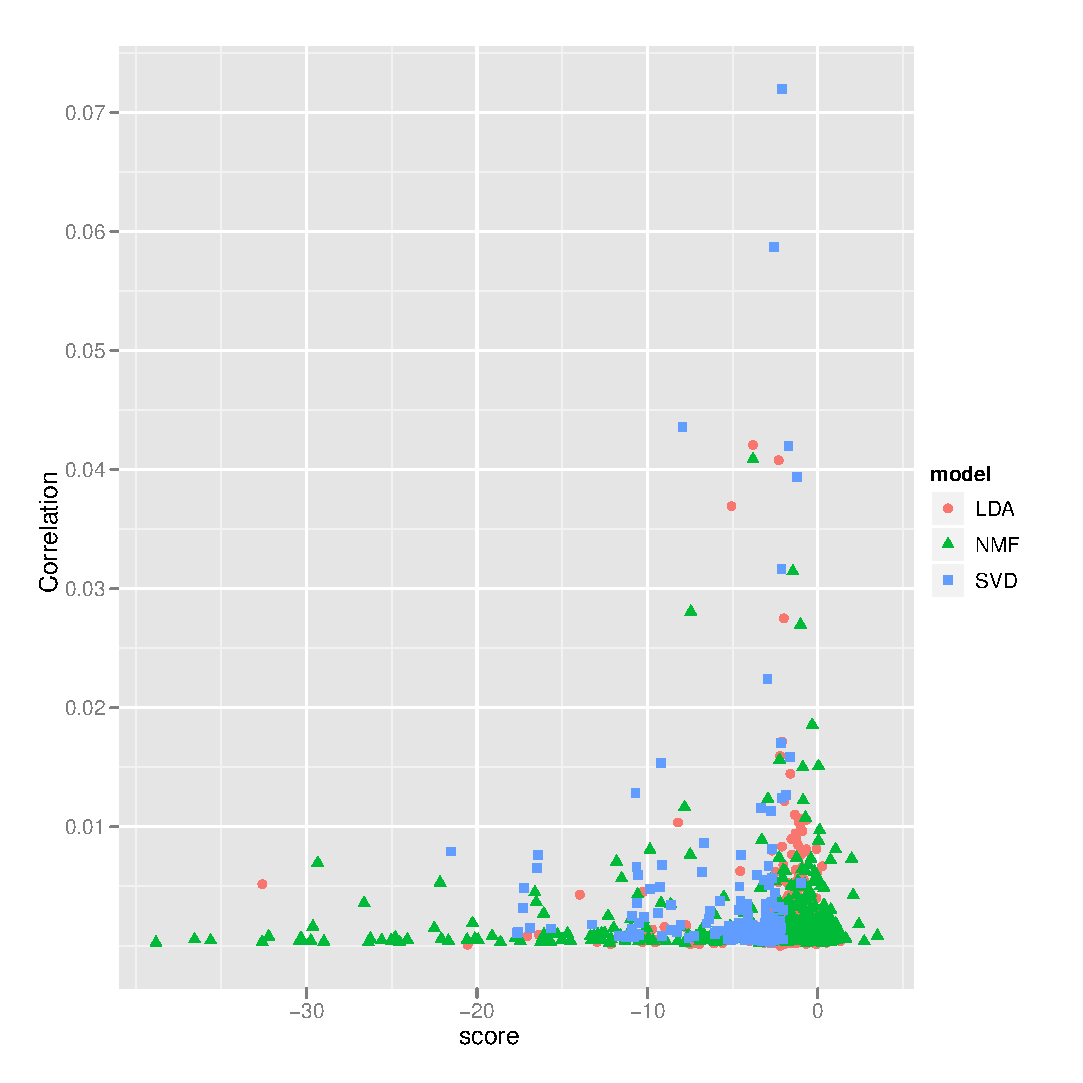
\includegraphics[width=.50\textwidth,height=.35\textwidth]{plots/uciNoSmoothing-rank-500.eps}}
  \caption{Comparison between topic coherence and topic rank with 500 topics}
  \label{fig:ranks500}
\end{figure*}

The initial evaluations for each coherence measure asked human judges to
directly evaluate topics \cite{newman10uci,mimno11umass}.  We expand upon this
comparison to human judgments by considering word similarity tasks that have
often been used to evaluate distributional semantic spaces
\cite{jurgens10sspace}.  Here, we use the learned topics as generalized
semantics describing our knowledge about words.  If a model's topics generalize
the knowledge accurately, we would expect similar words, such as ``cat'' and
``dog'', to be represented with a similar set of topics.  Rather than evaluating
individual topics, this similarity task considers the knowledge within the
entire set of topics, the topics act as more compact representation for the
known words in a corpus.

We use the \newcite{rubenstein65wordsim} and \newcite{finkelstein02relatedness}
word similarity tasks.  In each task, human judges were asked to evaluate the
similarity or relatedness between different sets of word pairs.   Fifty-One
Evaluators for the \newcite{rubenstein65wordsim} dataset were given 65 pairs of
words and asked to rate their similarity on a scale from 0 to 4, where a higher
score indicates a more similar word pair.  \newcite{finkelstein02relatedness}
broadens the word similarity evaluation and asked 13 to 16 different subjects
to rate 353 word pairs on a scale from 0 to 10 based on their relatedness, where
relatedness includes similarity and other semantic relations.  We can evaluate
each topic model by computing the cosine similarity between each pair of words
in the evaluate set and then compare the model's ratings to the human ratings by
ranked correlation.  A high correlation signifies that the topics closely model
human judgments.  

Figure \ref{fig:wordsim} displays the results.  SVD and LDA both surpass NMF on
the Rubenstein \& Goodenough test while SVD is clearly the best model on the
Finklestein et. al test.  While our first experiment showed that SVD was the
worst model in terms of topic coherence scores, this experiment indicates that
SVD provides an accurate, stable, and reliable approximation to human judgements
of similarity and relatedness between word pairs in comparison to other topic
models.

\subsection{Coherence versus Classification}

For our final experiment, we examine the relationship between topic
coherence and classification accuracy for each topic model.  We suspect that
highly coherent topics, and coherent topic models, will perform better for
classification.  We address this question by performing a document
classification task using the topic representations of documents as input features
and examine the relationship between topic coherence and the usefulness of the
corresponding feature for classification.

We trained each topic model with all 92,600 New York Times articles as before.
We use the section labels provided for each article as class labels, where each
label indicates the on-line section(s) under which the article was published and
should thus be related to the topics contained in each article.  To reduce the
noise in our data set we narrow down the articles to those that have only one
label and whose label is applied to at least 2000 documents.   This results in
57,696 articles with label distributions listed in Table \ref{tab:labels}.  We
then represent each document using columns in the topic by document matrix $H$
learned for each topic model.

\begin{table}[htbp]
  \centering
  \begin{tabular}{lr|lr}
    Label & Count & Label & Count \\ \hline
    New York and Region & 11219 &  U.S. & 3675	\\   
    Paid Death Notices & 11152 &   Arts & 3437	\\   
    Opinion & 8038 &               World & 3330	\\   
    Business & 7494 &              Style & 2137	\\   
    Sports & 7214 
  \end{tabular}
  \caption{Section label counts for New York Times articles used for
  classification}
  \label{tab:labels}
\end{table}

For each topic model trained on N topics, we performed stratified 10-fold
cross-validation on the 57,696 labeled articles. In each fold,
we build an automatically-sized bagged ensemble of unpruned CART-style decision
trees\cite{banfield07compareensemble} on 90\% of the
dataset\footnote{The precise choice of the classifier scheme matters
little, as long as it is accurate, speedy, and robust to label noise;
all of which is true of the choice here.}, use that ensemble
to assign labels to the other 10\%, and measure the accuracy of that assignment.
Figure \ref{fig:predict} shows the average classification accuracy over all ten
folds for each model.  Interestingly, SVD has slightly, but statistically
significantly, higher accuracy results than both NMF and LDA.  Furthermore,
performance quickly increases and plateaus with well under 50 topics.

Our bagged decision trees can also determine the importance of each feature
during classification.  We evaluate the strength of each topic during
classification by tracking the number of times each node in our decision trees
observe each topic, please see \cite{Caruana06miningcitizen} for more details.
Figure \ref{fig:ranks500} plot the relationship between this feature ranking and
the topic coherence for each topic when training LDA, SVD, and NMF on 500
topics.  Most topics for each model provide little classification information,
but SVD shows a much higher rank for several topics with a relatively higher
coherence score.  Interestingly, for all models, the most coherent topics are
not the most informative.  Figure \ref{fig:topic-ranks} plots a more compact
view of this same relationship: the Spearman rank correlation between
classification feature rank and topic coherence.  NMF shows the highest
correlation between rank and coherence, but none of the models show a high
correlation when using more than 100 topics.  SVD has the lowest
correlation, which is probably due to the model's overall low coherence yet high
classification accuracy.  



\section{Discussion and Conclusion}
\label{sec:discusssion}
Through our experiments, we made several exciting and interesting discoveries.
First, we discovered that the coherence metrics depend heavily on the smoothing
factor $\epsilon$.  The original value, $1.0$ created a positive bias towards
NMF from both metrics even when NMF generated incoherent topics.  The high
smoothing factor also gave a significant increase to SVD scores.  We suspect
that this was not an issue in previous studies with the coherence measures as
LDA prefers to form topics from words that co-occur frequently, whereas NMF and
SVD have no such preferences and often create low quality topics from completely
unrelated words.  Therefore, we suggest a smaller $\epsilon$ value in general.

We also found that the UCI measure often agreed with the UMass measure, but the
UCI-entropy aggregate method induced more separation between LSA, SVD, and NMF
in terms of topic coherence.  This measure also revealed the importance of the
smoothing factor for topic coherence measures.

With respects to human judgements, we found that coherence scores do not always
indicate a better representation of distributional information.  The SVD model
consistently out performed both LDA and NMF models, which each had higher
coherence scores, when attempting to predict human judgements of similarity.  

Lastly, we found all models capable of producing topics that improved document
classification.  At the same time, SVD provided the most information during
classification and outperformed the other models, which again had more coherent
topics.  Our comparison between topic coherence scores and feature importance in
classification revealed that relatively high quality topics, but not the most
coherent topics, drive most of the classification decisions, and most topics do
not affect the accuracy.  

Overall, we see that each topic model paradigm has it's own strengths and
weaknesses.  Latent Semantic Analysis with Singular Value Decomposition fails to
form individual topics that aggregate similar words, but it does remarkably well
when considering all the learned topics as similar words develop a similar topic
representation.  These topics similarly perform well during classification.
Conversely, both Non Negative Matrix factorization and Latent Dirichlet
Allocation learn concise and coherent topics and achieved similar performance on
our evaluations. However, NMF learns more incoherent topics than LDA and SVD.
For applications in which a human end-user will interact with learned topics,
the flexibility of LDA and the coherence advantages of LDA warrant strong
consideration.  All of code for this work will be made available through an open
source project.\footnote{https://github.com/fozziethebeat/TopicModelComparison}


\section{Acknowledgments}

This work was performed under the auspices of the U.S. Department of Energy by
Lawrence Livermore National Laboratory under Contract DE-AC52-07NA27344
(LLNL-CONF-522871) and by Sandia National Laboratory under Contract
DE-AC04-94AL85000.

\bibliographystyle{acl2012}
\bibliography{topic_coherence}

\end{document}
